% !TeX root = ../../main.tex
% Chương 4: Kết quả và Phân tích

\chapter{Kết quả và Phân tích}

Chương này trình bày kết quả benchmark theo từng kịch bản đã mô tả ở Chương 3. Mạch phân tích bắt đầu từ kịch bản đo và mức tải, sau đó đọc kết quả, diễn giải xu hướng và rút ra kết luận. Các bảng và biểu đồ là kết quả hậu xử lý từ các lần chạy benchmark, giúp việc đọc kết quả có hệ thống hơn.

Trọng tâm của chương là trả lời ba câu hỏi: mỗi kịch bản kiểm tra điều gì, kết quả chính là gì và có thể kết luận đến mức nào. Các thống kê như khoảng tin cậy 95\%, delta \%, giá trị \(p\) theo kiểm định kiểu Welch và CV\% được dùng như bằng chứng hỗ trợ.

Trong chương này, một kết quả được xem là có ý nghĩa thống kê khi \(p < 0.05\), tức là dữ liệu hiện tại đủ mạnh để bác bỏ giả thuyết không \(H_0\) ở mức ý nghĩa 5\%. Với so sánh A/B, \(H_0\) được hiểu là hai nhóm không khác biệt đáng kể về trung bình của metric đang xét. Tuy nhiên, do nhiều nhóm đo chỉ có \(n=3\), ý nghĩa thống kê chỉ được dùng như bằng chứng hỗ trợ và phải đọc cùng delta \%, khoảng tin cậy 95\% và bối cảnh kịch bản.

\section{Hiệu chuẩn tải và lựa chọn mức tải}

Hiệu chuẩn tải được thực hiện trước benchmark chính để chọn các mức tải phù hợp. Nếu tải quá thấp, khác biệt giữa hai mode có thể bị che khuất. Nếu tải quá cao, kết quả có thể bị chi phối bởi stress cực đoan. Vì vậy, L1, L2 và L3 được chọn từ dữ liệu hiệu chuẩn thay vì chọn thủ công.

Hình~\ref{fig:calibration-curve} biểu diễn p99 latency theo target QPS trong lượt quét hiệu chuẩn. P99 được dùng vì phần đuôi độ trễ thường nhạy hơn với queueing, scheduling, connection handling và chi phí xử lý Service. Các đường dọc trong hình chỉ đánh dấu L1, L2 và L3; chúng không phải error bars.

\begin{figure}[H]
    \centering
    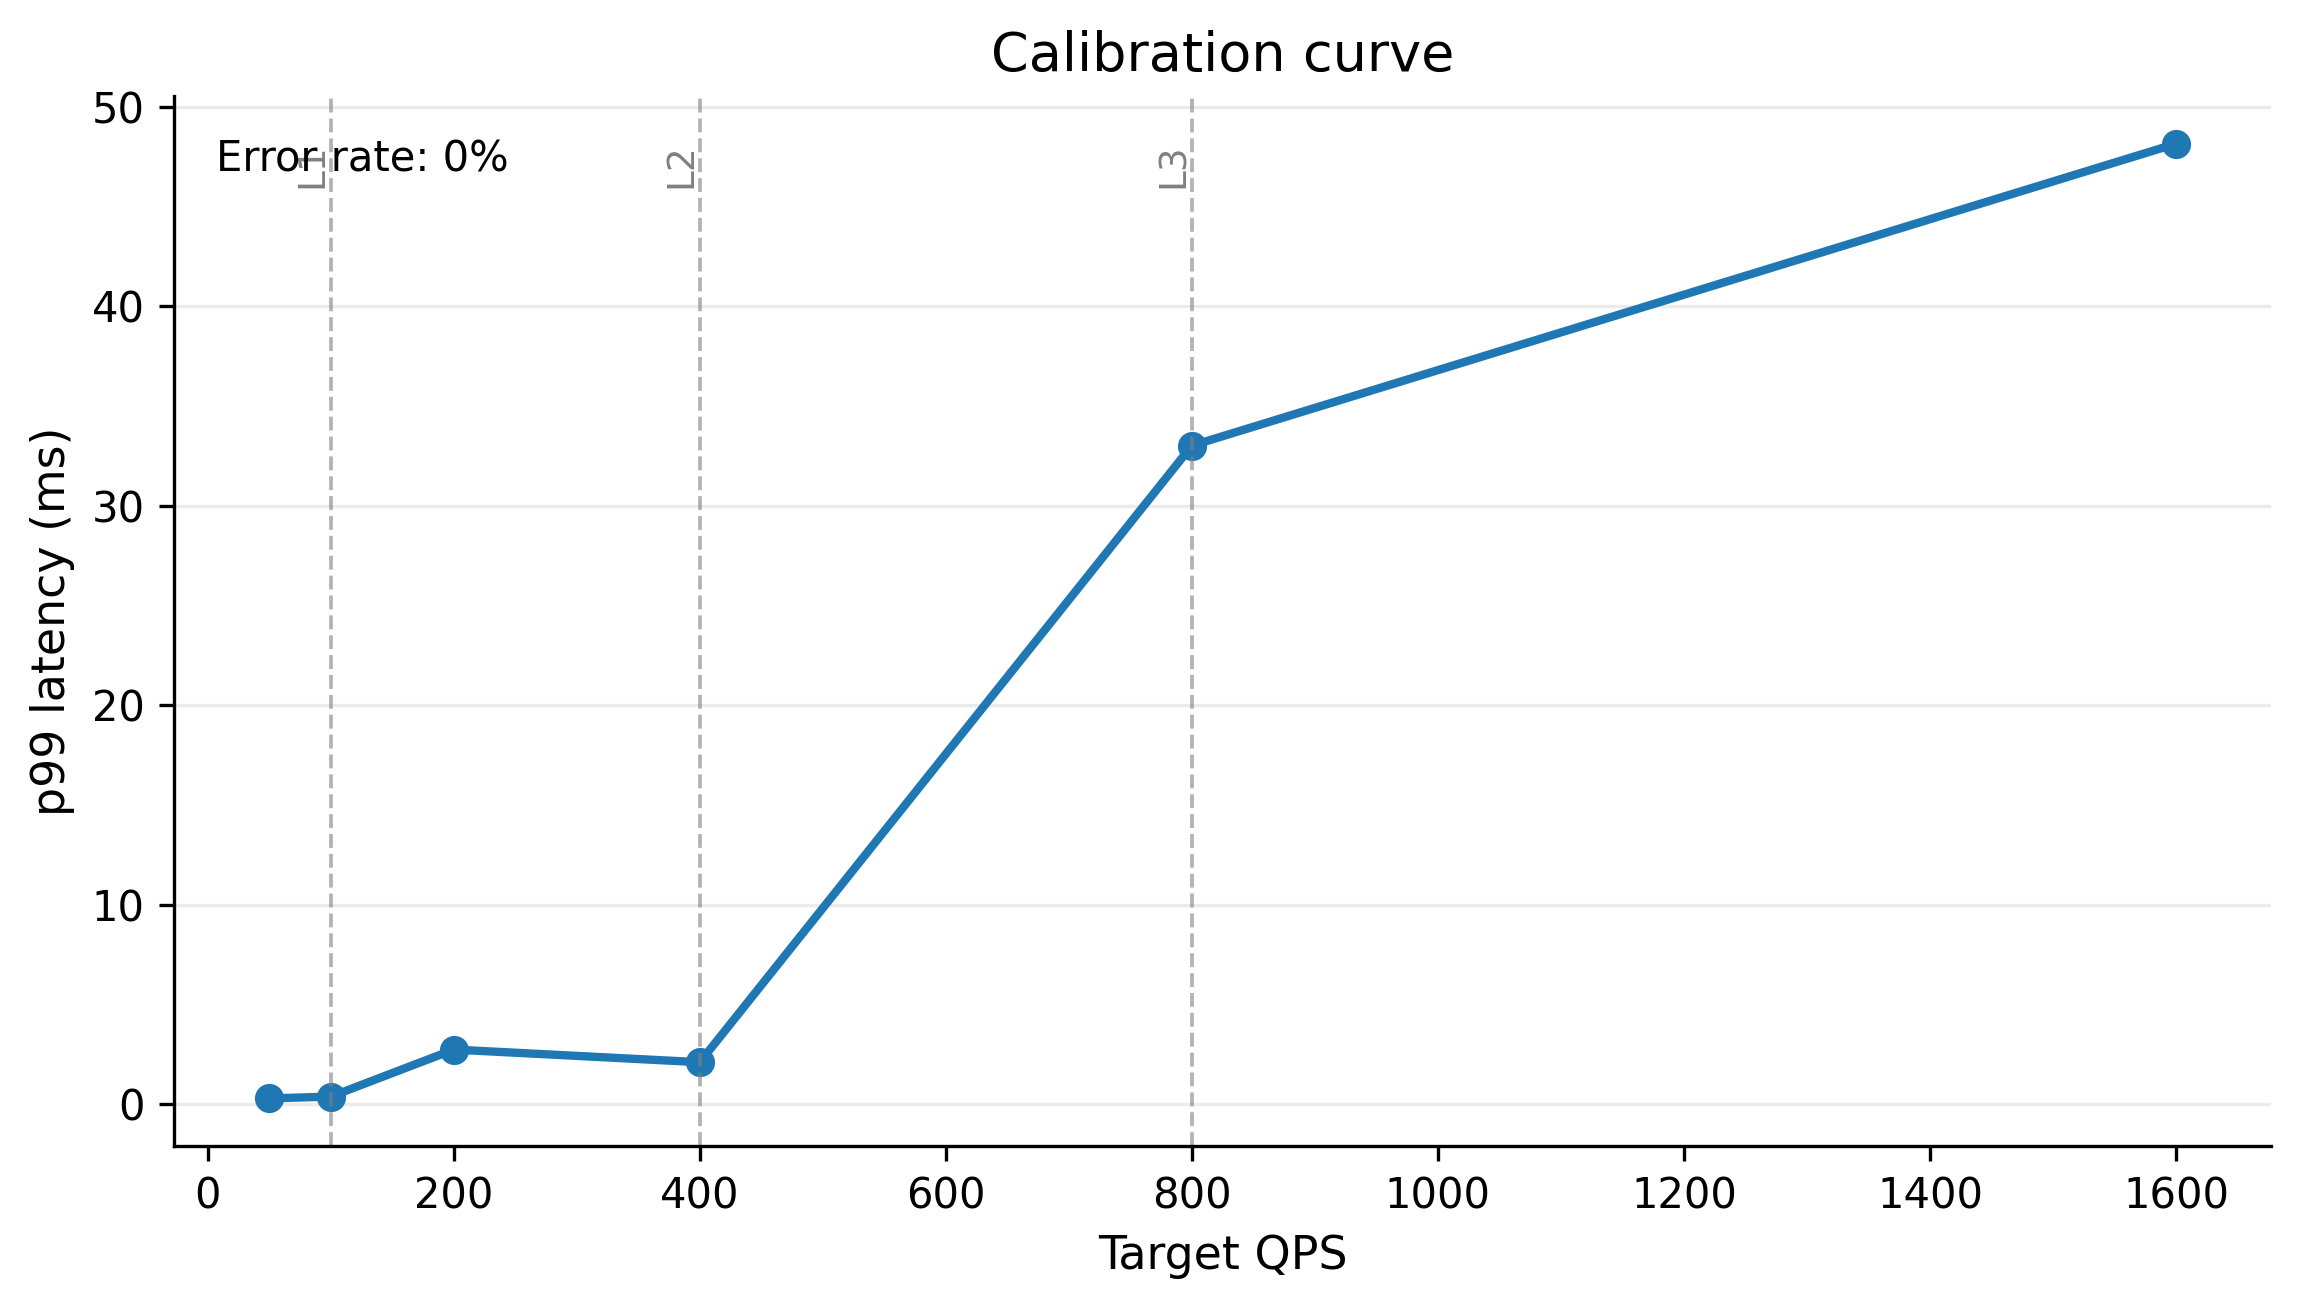
\includegraphics[width=0.90\textwidth]{../figures/thesis/fig-calibration-curve.png}
    \caption{Đường hiệu chuẩn tải và lựa chọn L1, L2, L3; các đường dọc chỉ là mốc tải, không phải thanh sai số}
    \label{fig:calibration-curve}
\end{figure}

\begin{table}[H]
\centering
\caption{Tóm tắt các điểm hiệu chuẩn tải}
\label{tab:calibration-load-selection}
\renewcommand{\arraystretch}{1.2}
\begin{tabularx}{\textwidth}{>{\raggedleft\arraybackslash}p{1.2cm}>{\raggedleft\arraybackslash}p{1.3cm}>{\raggedleft\arraybackslash}p{1.5cm}>{\raggedleft\arraybackslash}p{1.5cm}>{\raggedleft\arraybackslash}p{1.7cm}>{\raggedleft\arraybackslash}p{1.7cm}>{\raggedright\arraybackslash}X}
\toprule
\textbf{QPS} & \textbf{Conns} & \textbf{p50} & \textbf{p90} & \textbf{p99} & \textbf{Lỗi} & \textbf{Vai trò} \\
\midrule
100 & 8 & 0.208 ms & 0.353 ms & 0.385 ms & 0.000\% & L1, tải nhẹ \\
400 & 32 & 0.846 ms & 1.854 ms & 2.107 ms & 0.000\% & L2, tải trung bình \\
800 & 64 & 1.709 ms & 4.411 ms & 33.006 ms & 0.000\% & L3, tải cao có p99 tăng rõ \\
1600 & 64 & 3.085 ms & 5.746 ms & 48.135 ms & 0.000\% & Điểm stress cao hơn, không dùng làm L3 cuối \\
\bottomrule
\end{tabularx}
\end{table}

\textbf{Phân tích.} Kết quả hiệu chuẩn cho thấy 100 QPS phù hợp làm L1 vì p99 thấp và ổn định. Mức 400 QPS được chọn làm L2 vì tail latency bắt đầu rõ hơn nhưng chưa tạo lỗi HTTP. Mức 800 QPS được chọn làm L3 vì p99 tăng mạnh lên khoảng 33.006 ms, trong khi achieved RPS vẫn gần target và error rate vẫn bằng 0\%.

Như vậy, 800 QPS đủ làm phần đuôi độ trễ nhạy hơn mà chưa biến phép đo thành tình huống lỗi hàng loạt. Điểm 1600 QPS không được chọn làm L3 vì có thể làm các pha burst của S2 quá cực đoan. Do đó, L3 nên được hiểu là mức tải cao làm lộ rõ tail latency, không phải điểm bão hòa tuyệt đối.

\textbf{Kết luận.} Error rate bằng 0\% chỉ cho thấy request không lỗi HTTP trong phạm vi đo; nó không có nghĩa hệ thống không chịu áp lực. Sự tăng mạnh của p99 tại 800 QPS là cơ sở để xem L3 là mức tải cao có ý nghĩa phân tích. Vì vậy, L1/L2/L3 phù hợp để dùng cho benchmark chính.

\section{Kết quả S1: tải ổn định}

S1 so sánh Mode A và Mode B trong điều kiện service traffic ổn định. Đây là kịch bản sạch nhất để quan sát khác biệt datapath vì không có burst, không thay đổi policy OFF/ON và không cố ý tạo connection churn. Metric chính là p99 latency vì benchmark tập trung vào tail latency.

Các biểu đồ chính của S1 gồm p99 theo mức tải, so sánh p50/p90/p99 và delta p99 của Mode B so với Mode A. Ba hình này lần lượt cho biết xu hướng tail latency, xu hướng ở nhiều percentile và độ lớn chênh lệch theo phần trăm.

\begin{figure}[H]
    \centering
    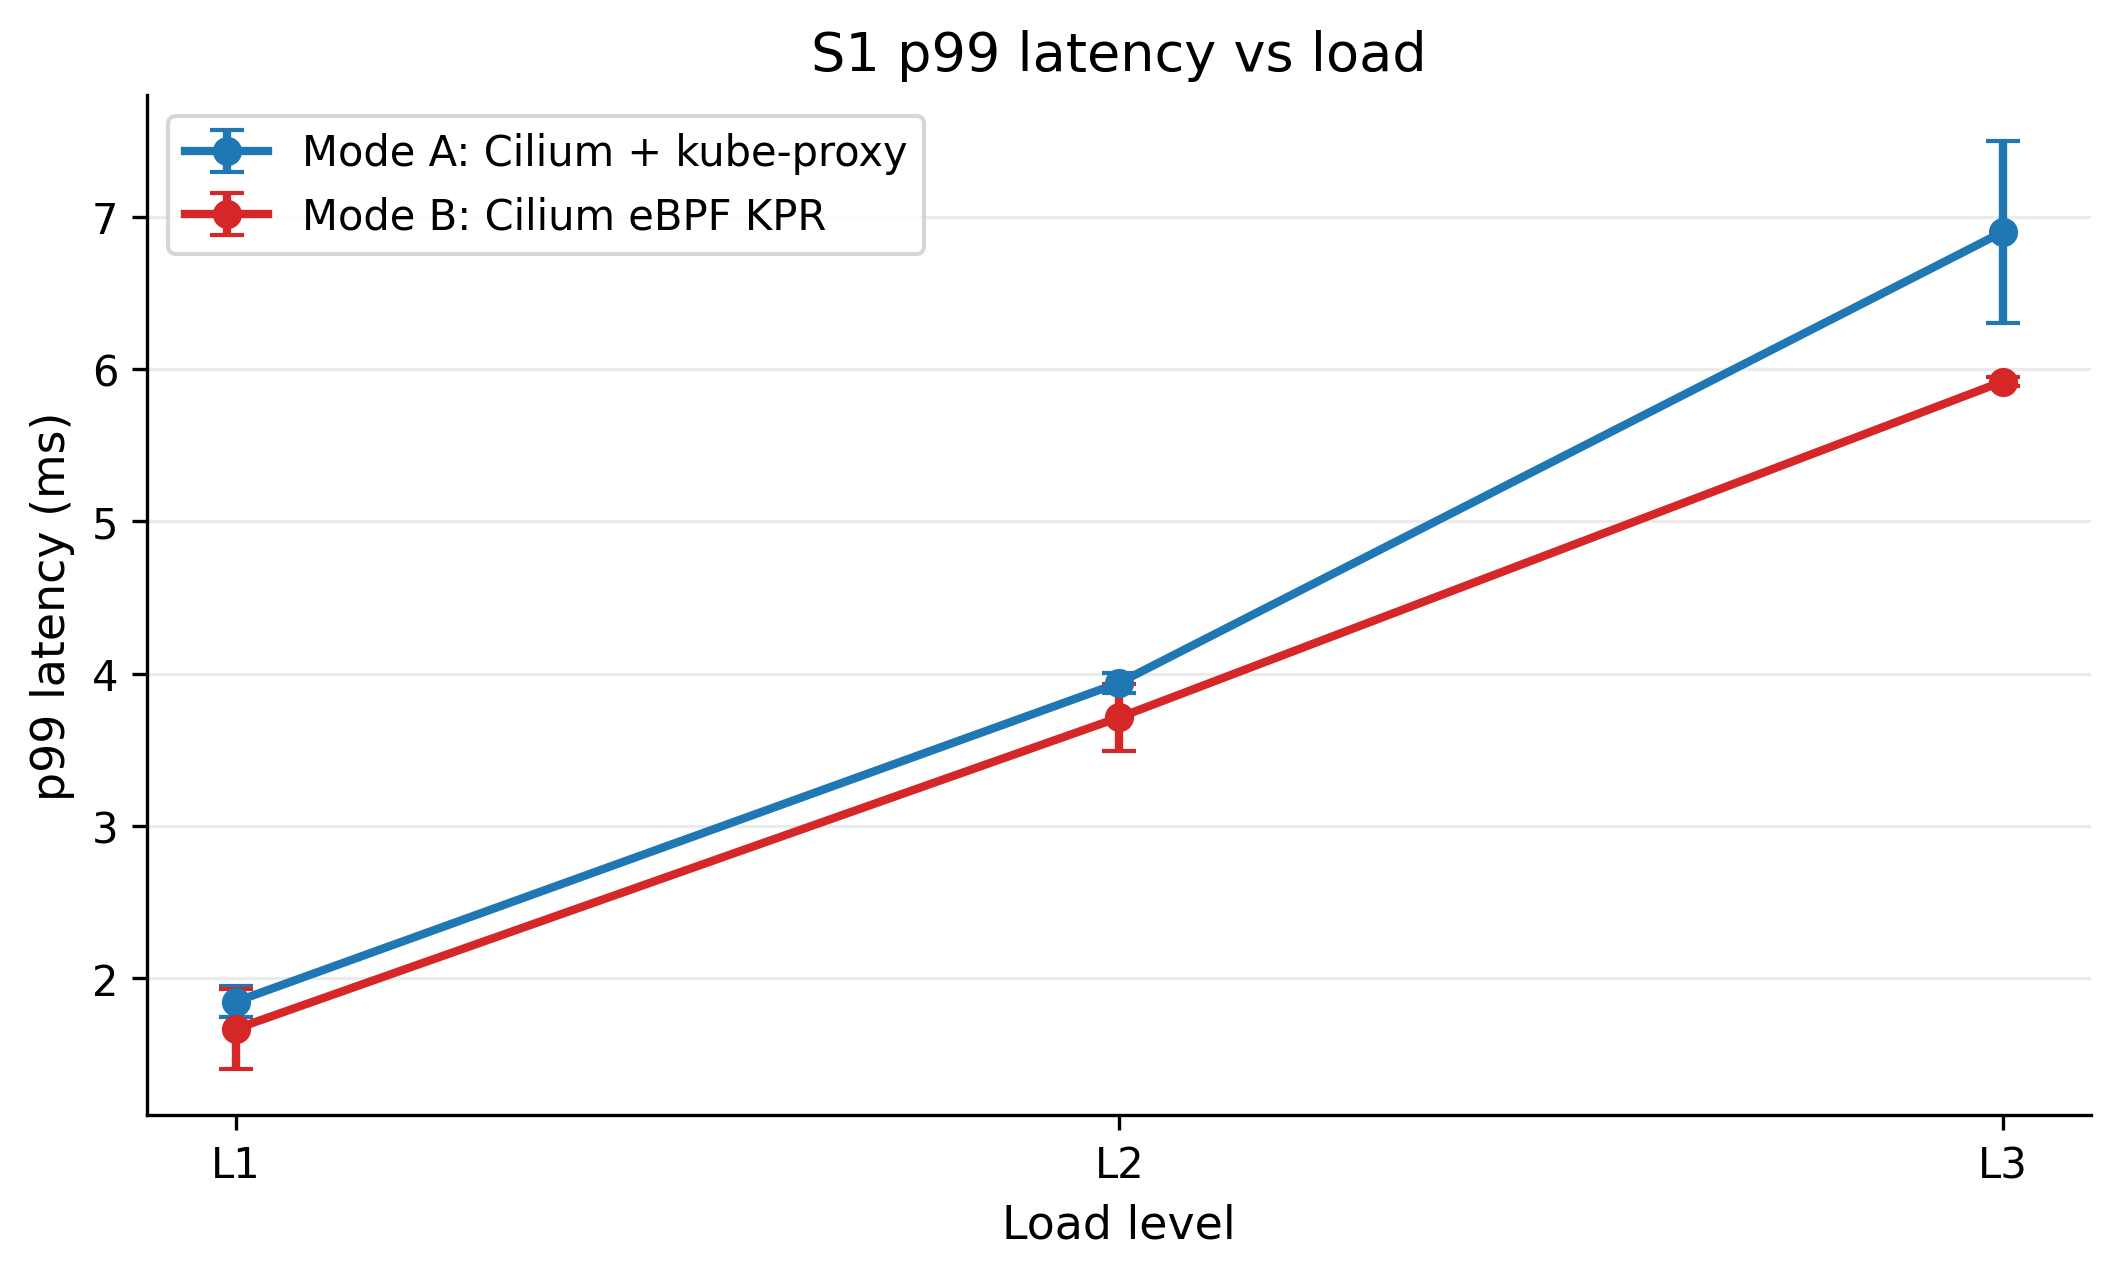
\includegraphics[width=0.90\textwidth]{../figures/thesis/fig-s1-p99-vs-load.png}
    \caption{P99 latency của S1 theo mức tải; các vạch dọc biểu diễn khoảng tin cậy 95\% quanh giá trị trung bình}
    \label{fig:s1-p99-vs-load}
\end{figure}

\begin{table}[H]
\centering
\caption{So sánh p99 latency trong S1}
\label{tab:s1-p99-summary}
\renewcommand{\arraystretch}{1.2}
\begin{tabularx}{\textwidth}{>{\raggedright\arraybackslash}p{1.2cm}>{\raggedleft\arraybackslash}p{2.0cm}>{\raggedleft\arraybackslash}p{2.0cm}>{\raggedleft\arraybackslash}p{2.0cm}>{\raggedleft\arraybackslash}p{1.5cm}>{\raggedright\arraybackslash}X}
\toprule
\textbf{Tải} & \textbf{Mode A p99} & \textbf{Mode B p99} & \textbf{Delta B/A} & \textbf{\(p\)} & \textbf{Diễn giải} \\
\midrule
L1 & 1.846 ms & 1.667 ms & -9.702\% & 0.0838 & Xu hướng, chưa significant \\
L2 & 3.939 ms & 3.712 ms & -5.766\% & 0.0377 & Significant \\
L3 & 6.899 ms & 5.917 ms & -14.223\% & 0.0191 & Significant \\
\bottomrule
\end{tabularx}
\end{table}

\textbf{Phân tích.} Hình~\ref{fig:s1-p99-vs-load} cho thấy p99 của cả hai mode tăng theo tải. Mode B có p99 trung bình thấp hơn Mode A ở cả ba mức tải. Tuy nhiên, L1 chỉ nên xem là xu hướng vì chưa significant. L2 và L3 có bằng chứng mạnh hơn; riêng L3 có delta lớn nhất, khoảng -14.2\%, nên cũng có ý nghĩa thực tế rõ hơn.

\begin{figure}[H]
    \centering
    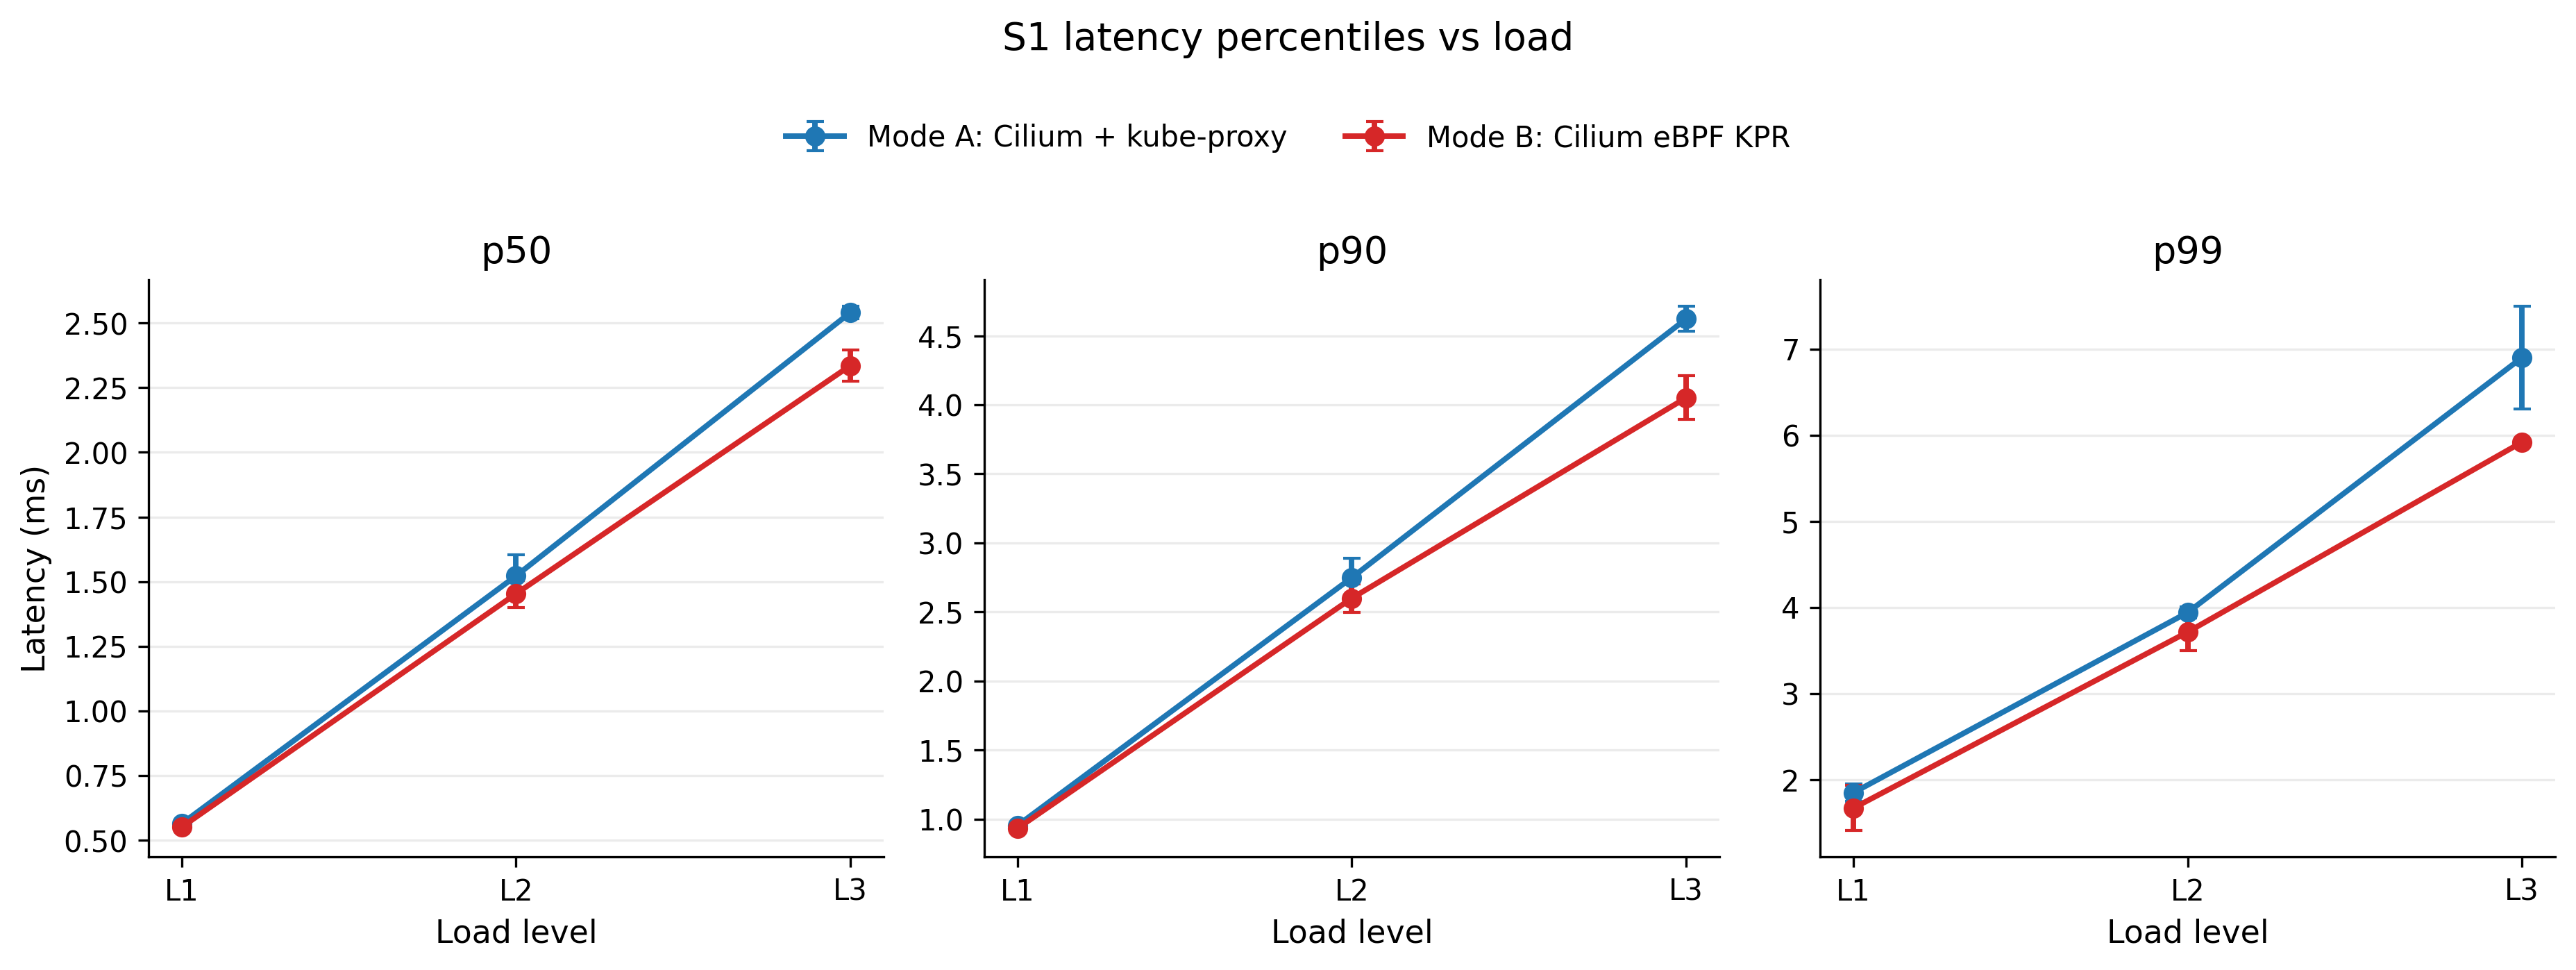
\includegraphics[width=0.90\textwidth]{../figures/thesis/fig-s1-latency-small-multiples.png}
    \caption{So sánh p50, p90 và p99 trong S1; các vạch dọc biểu diễn khoảng tin cậy 95\% quanh giá trị trung bình}
    \label{fig:s1-latency-small-multiples}
\end{figure}

Hình~\ref{fig:s1-latency-small-multiples} cho thấy ở L3, Mode B thấp hơn ở cả p50, p90 và p99. Vì xu hướng không chỉ xuất hiện ở một percentile đơn lẻ, kết quả S1 trở nên thuyết phục hơn.

\begin{figure}[H]
    \centering
    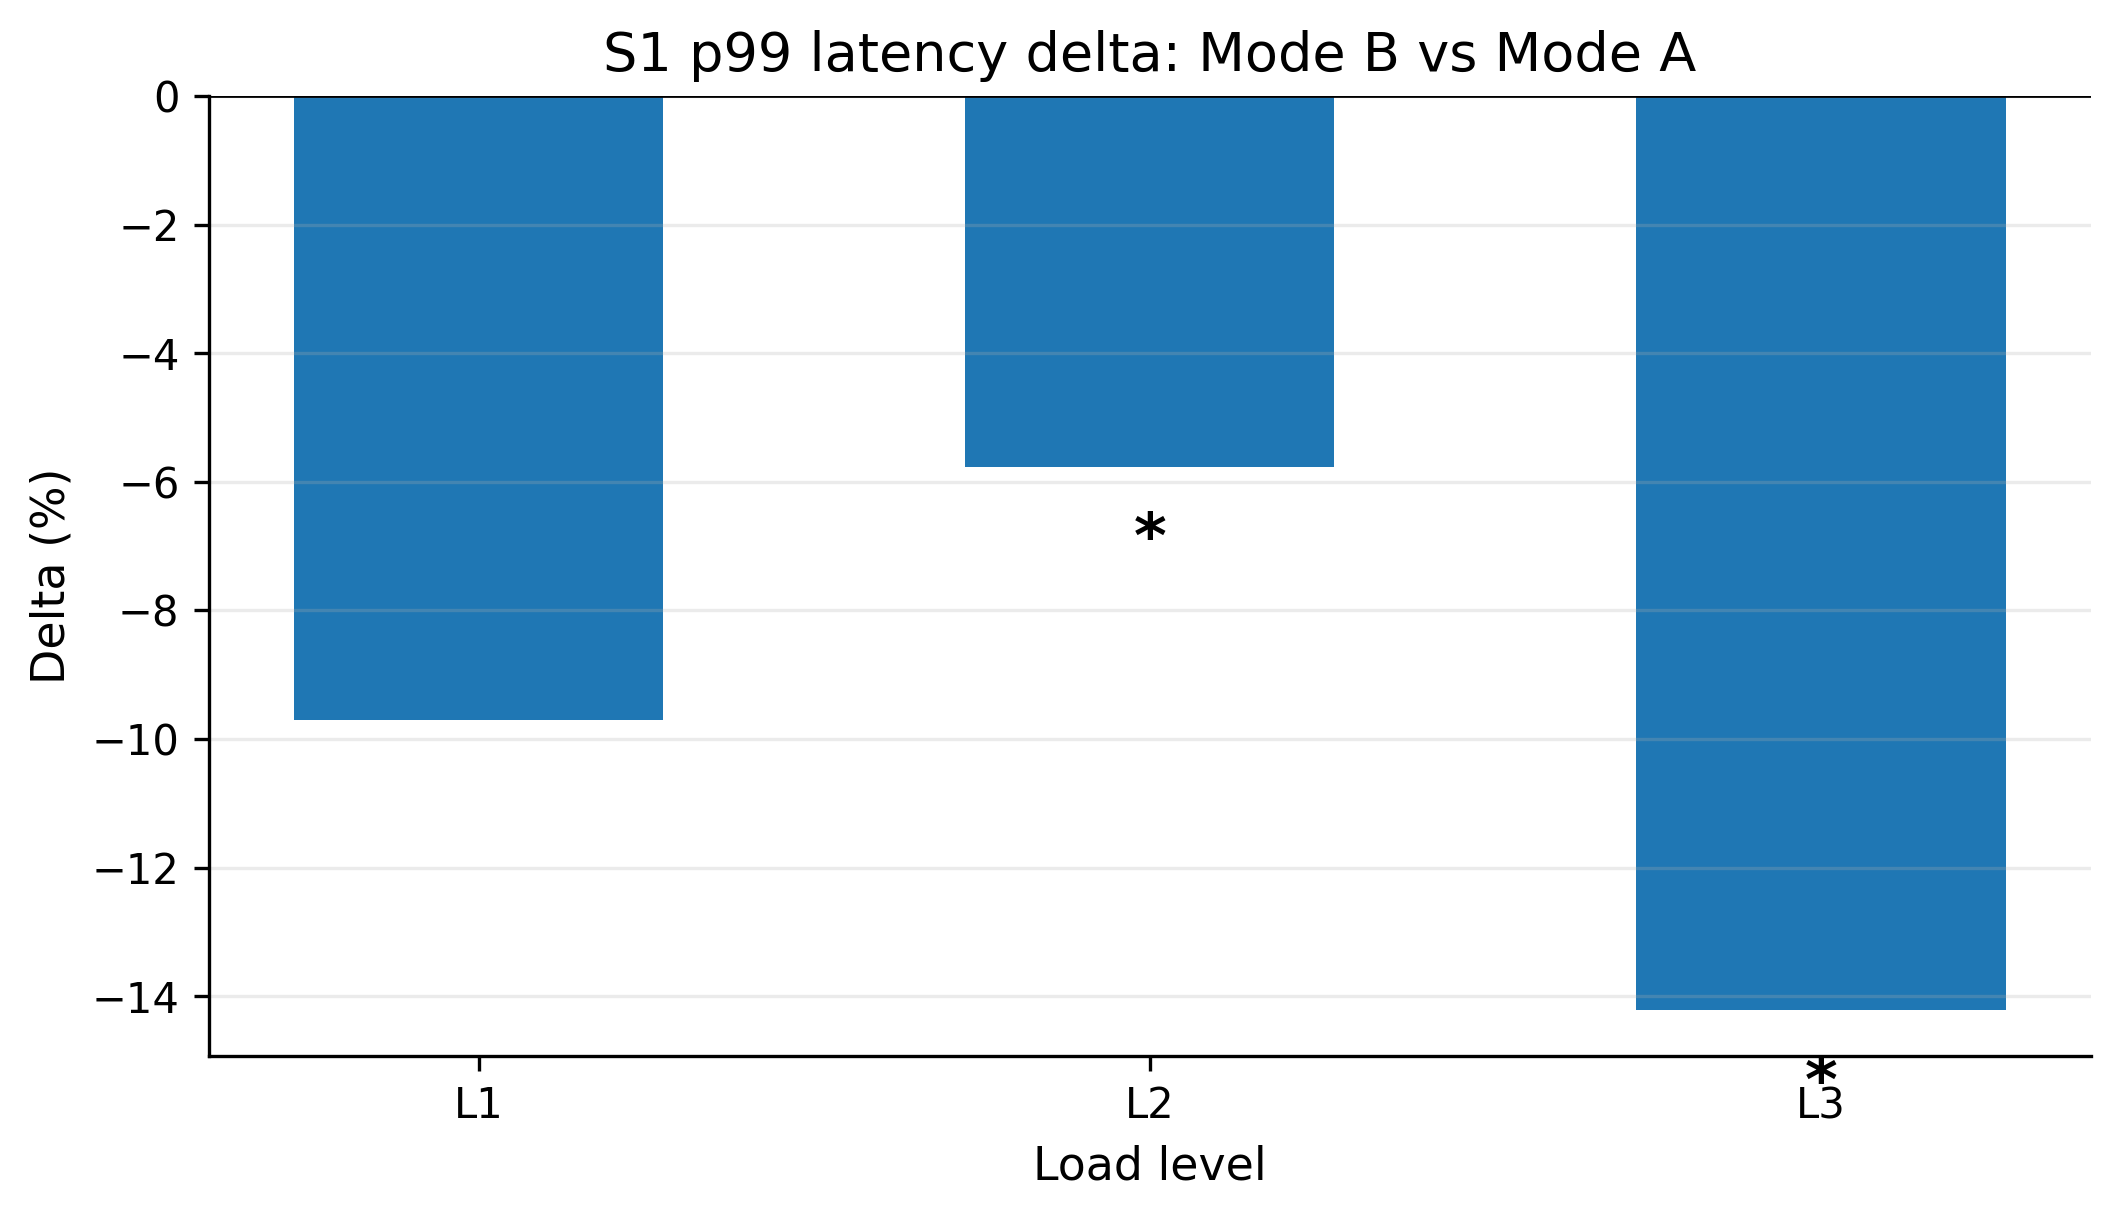
\includegraphics[width=0.82\textwidth]{../figures/thesis/fig-s1-delta-p99.png}
    \caption{Chênh lệch p99 của Mode B so với Mode A trong S1}
    \label{fig:s1-delta-p99}
\end{figure}

Hình~\ref{fig:s1-delta-p99} trình bày cùng kết quả dưới dạng delta phần trăm. Giá trị âm nghĩa là Mode B có p99 thấp hơn Mode A; điểm cần chú ý nhất là mức giảm tại L3.

Về cơ chế, S1 phù hợp để liên hệ kết quả với service datapath. Mode A dựa trên kube-proxy/iptables, DNAT và conntrack; Mode B dùng Cilium eBPF kube-proxy replacement. Khi tải tăng, chi phí nhỏ trên từng request dễ tích lũy ở phần đuôi, làm khác biệt p99 rõ hơn.

Hình~\ref{fig:s1-grafana-cpu-evidence} và Hình~\ref{fig:s1-grafana-memory-evidence} là bằng chứng vận hành hỗ trợ cho S1 L3. Hai hình dùng panel namespace-level để kiểm tra CPU và memory của namespace benchmark; các ảnh S1 L2 và bản phóng lớn được đặt ở Phụ lục~E.

Các ảnh không cho thấy dấu hiệu CPU hoặc memory pressure nghiêm trọng trong cửa sổ S1 L3. Vì đây chỉ là screenshot telemetry, chúng được dùng như sanity check, không phải bằng chứng định lượng để giải thích trực tiếp chênh lệch p99.

\begin{figure}[H]
    \centering
    \textbf{Mode A -- CPU namespace}\\[0.25em]
    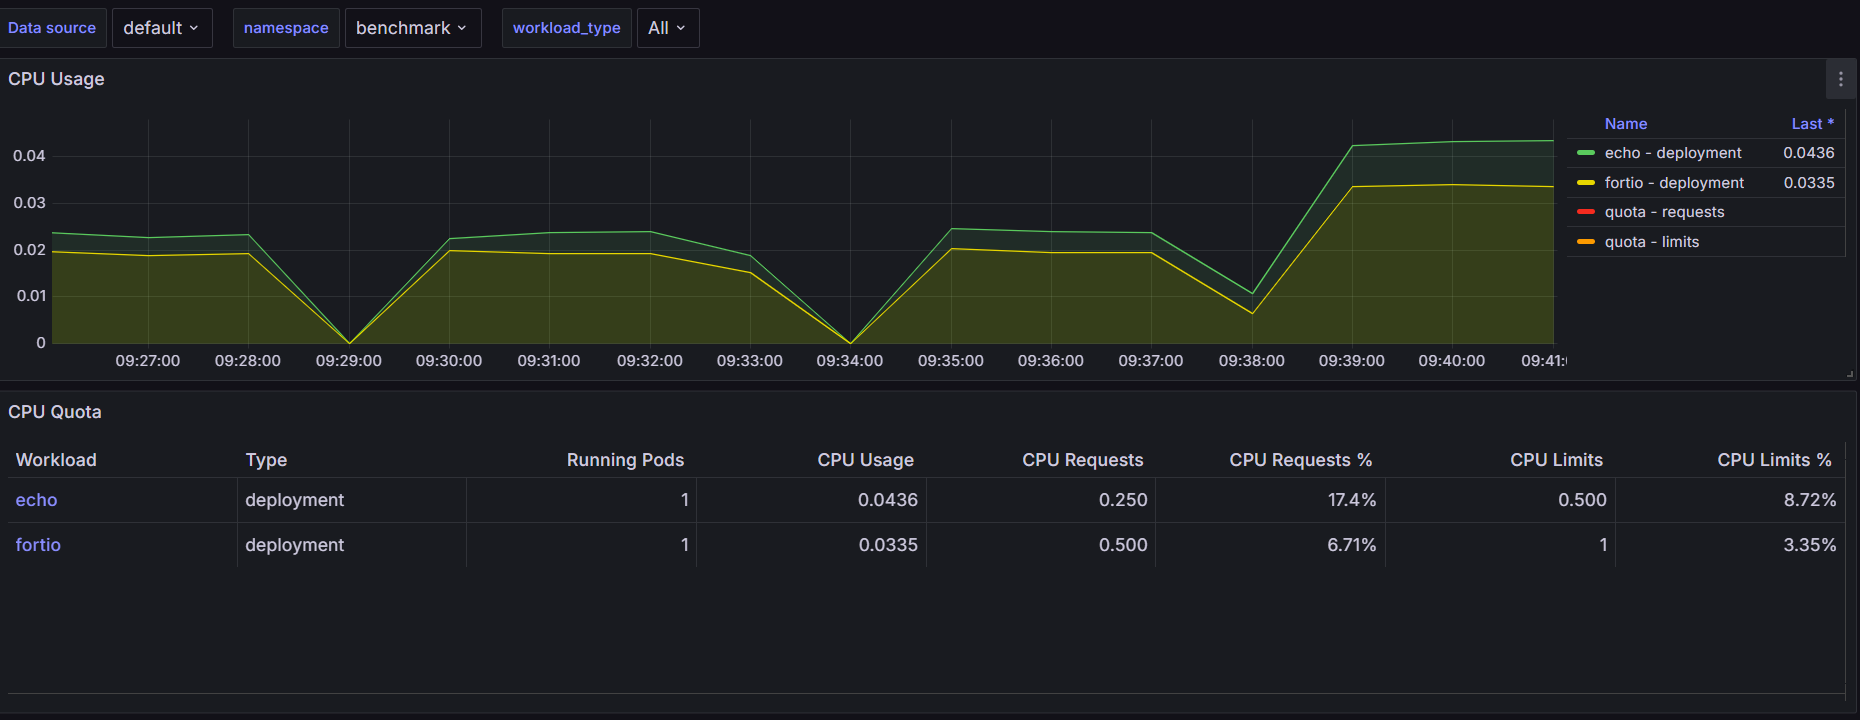
\includegraphics[width=0.88\textwidth]{../figures/grafana/modeA/grafana-ns-cpu-S1-L3-R1.png}
    \vspace{0.5em}
    
    \textbf{Mode B -- CPU namespace}\\[0.25em]
    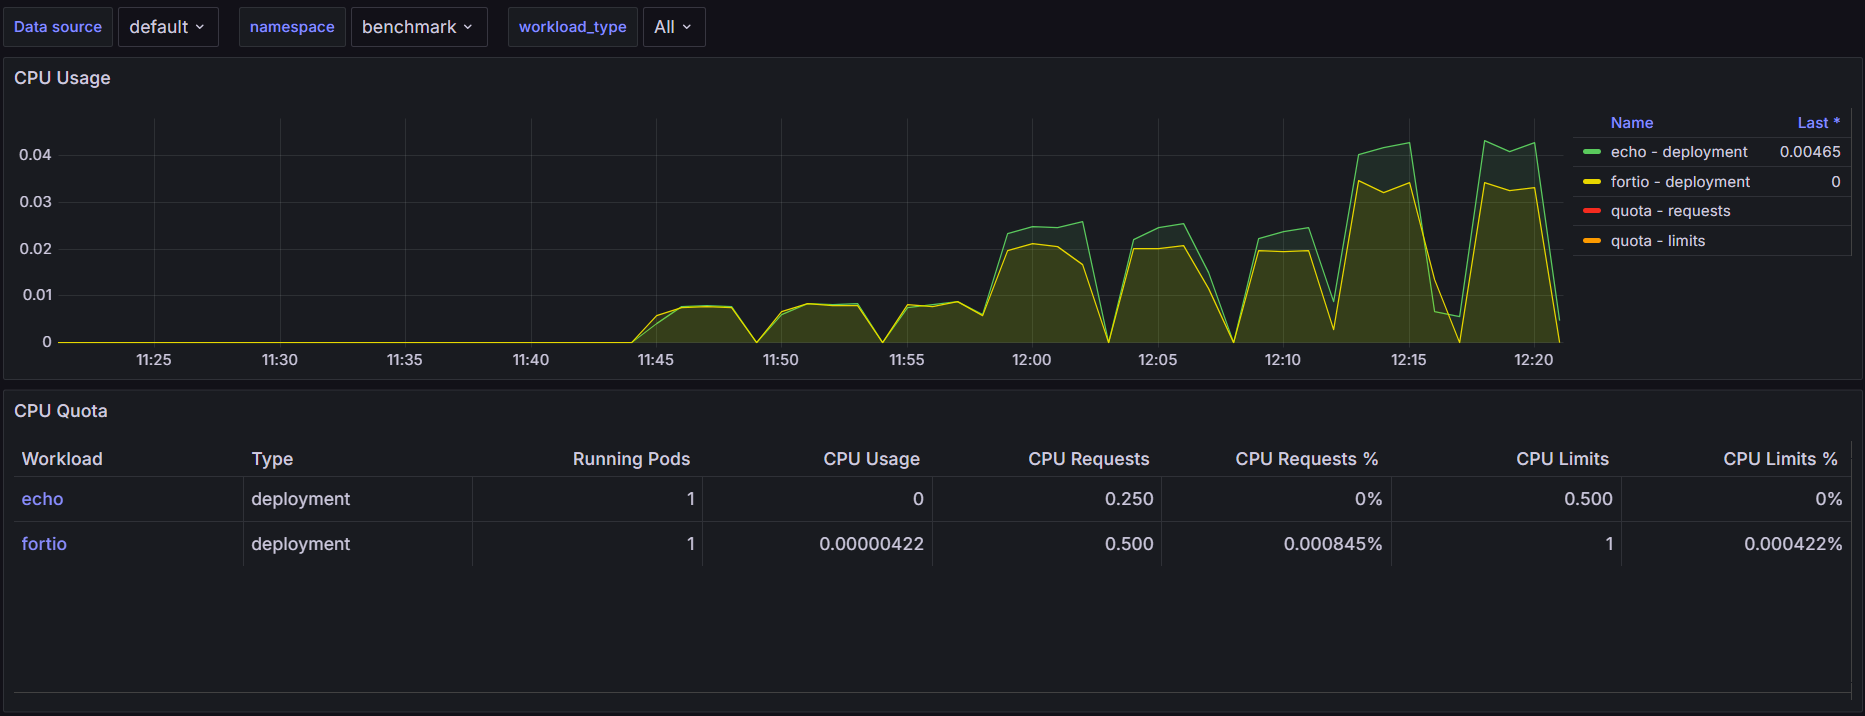
\includegraphics[width=0.88\textwidth]{../figures/grafana/modeB/grafana-ns-cpu-S1-L3.png}
    \caption{Bằng chứng Grafana namespace-level về CPU cho S1 L3 ở Mode A và Mode B; ảnh dùng để kiểm tra bối cảnh vận hành và không phải kết quả hiệu năng chính}
    \label{fig:s1-grafana-cpu-evidence}
\end{figure}

\begin{figure}[H]
    \centering
    \textbf{Mode A -- memory namespace}\\[0.25em]
    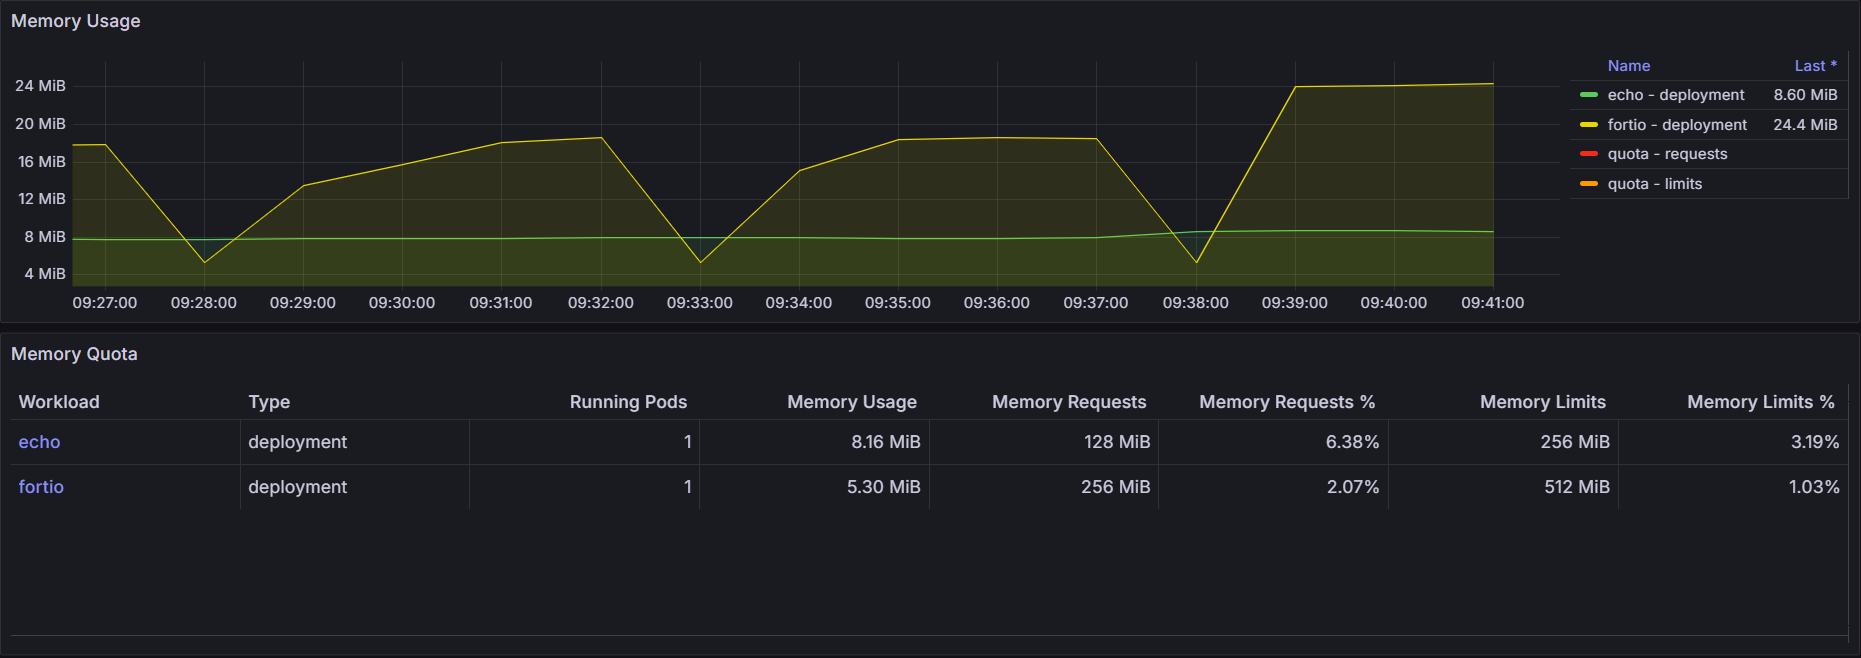
\includegraphics[width=0.88\textwidth]{../figures/grafana/modeA/grafana-ns-mem-S1-L3-R1.png}
    \vspace{0.5em}

    \textbf{Mode B -- memory namespace}\\[0.25em]
    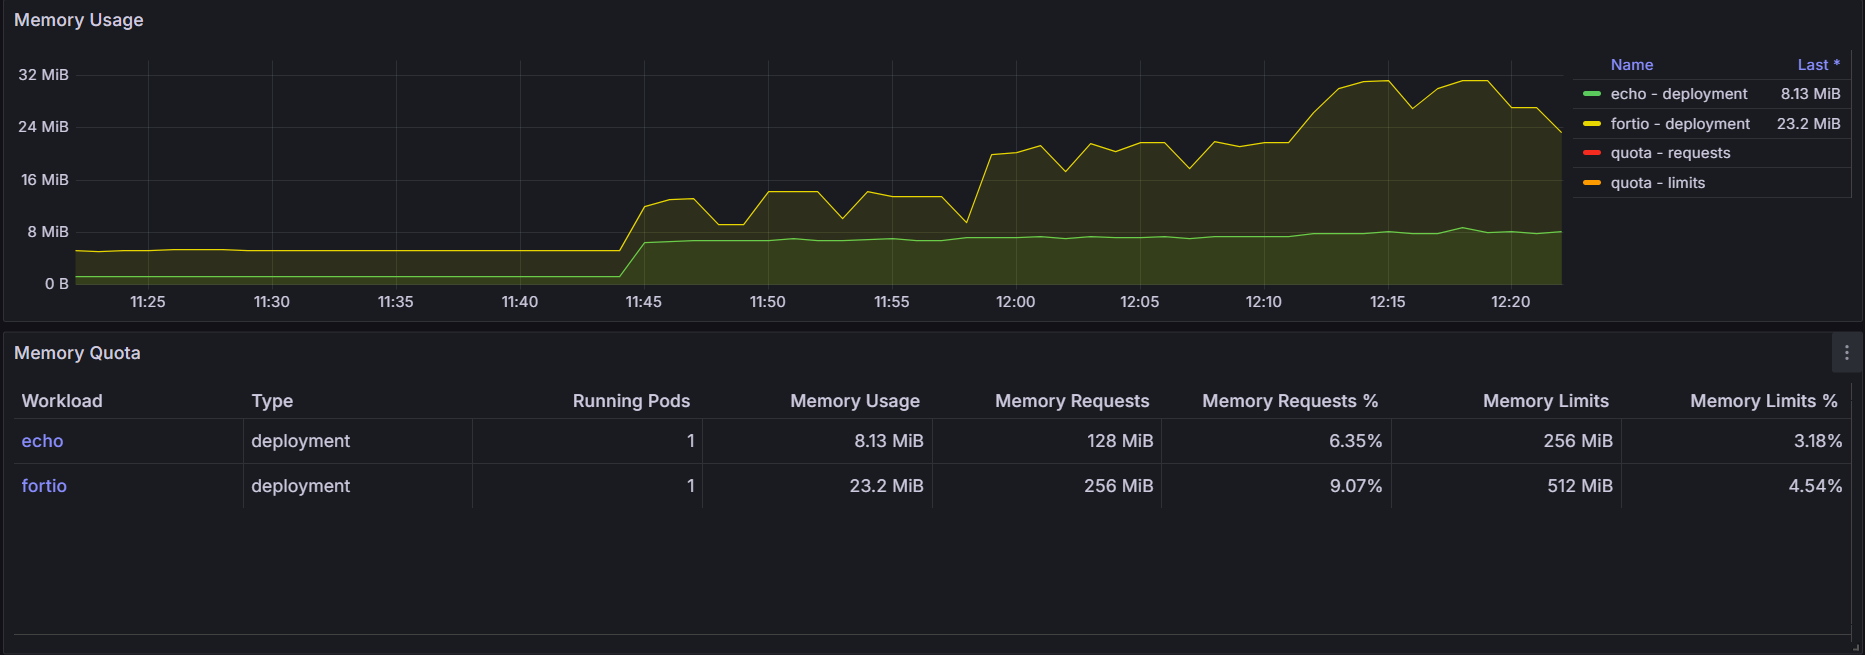
\includegraphics[width=0.88\textwidth]{../figures/grafana/modeB/grafana-ns-mem-S1-L3.png}
    \caption{Bằng chứng Grafana namespace-level về memory cho S1 L3 ở Mode A và Mode B; ảnh dùng để kiểm tra bối cảnh vận hành và không phải kết quả hiệu năng chính}
    \label{fig:s1-grafana-memory-evidence}
\end{figure}

\textbf{Kết luận.} Trong S1, Mode B cho thấy lợi thế p99 rõ hơn ở L2 và L3; L1 chỉ nên viết như xu hướng. Kết quả phù hợp với kỳ vọng về eBPF service datapath, nhưng không chứng minh Mode B luôn nhanh hơn trong mọi cluster hoặc workload.

\section{Kết quả S2: stress và thay đổi kết nối}

S2 kiểm tra hai mode dưới workload có nhiều pha, burst và connection churn. Kết quả không nên gộp thành một giá trị trung bình duy nhất, vì ramp-up, sustained, burst và cooldown tạo các trạng thái tải khác nhau. Cấu trúc này làm p99 nhạy hơn với trạng thái kết nối, cache, scheduling và dao động hệ thống.

Pipeline vẫn tổng hợp p50 và p90 cho S2, nhưng phần thân chương ưu tiên p99 vì mục tiêu chính là tail latency dưới burst và connection churn. Hai biểu đồ p99 theo pha là nguồn phân tích chính. Heatmap chỉ đóng vai trò tóm tắt hướng chênh lệch theo load và phase.

\subsection{S2 tại L2}

Hình~\ref{fig:s2-phase-p99-l2} cho thấy S2 tại L2 có kết quả pha trộn. Mode B thấp hơn Mode A ở phần lớn pha, nhưng không nhất quán trong toàn bộ run.

\begin{figure}[H]
    \centering
    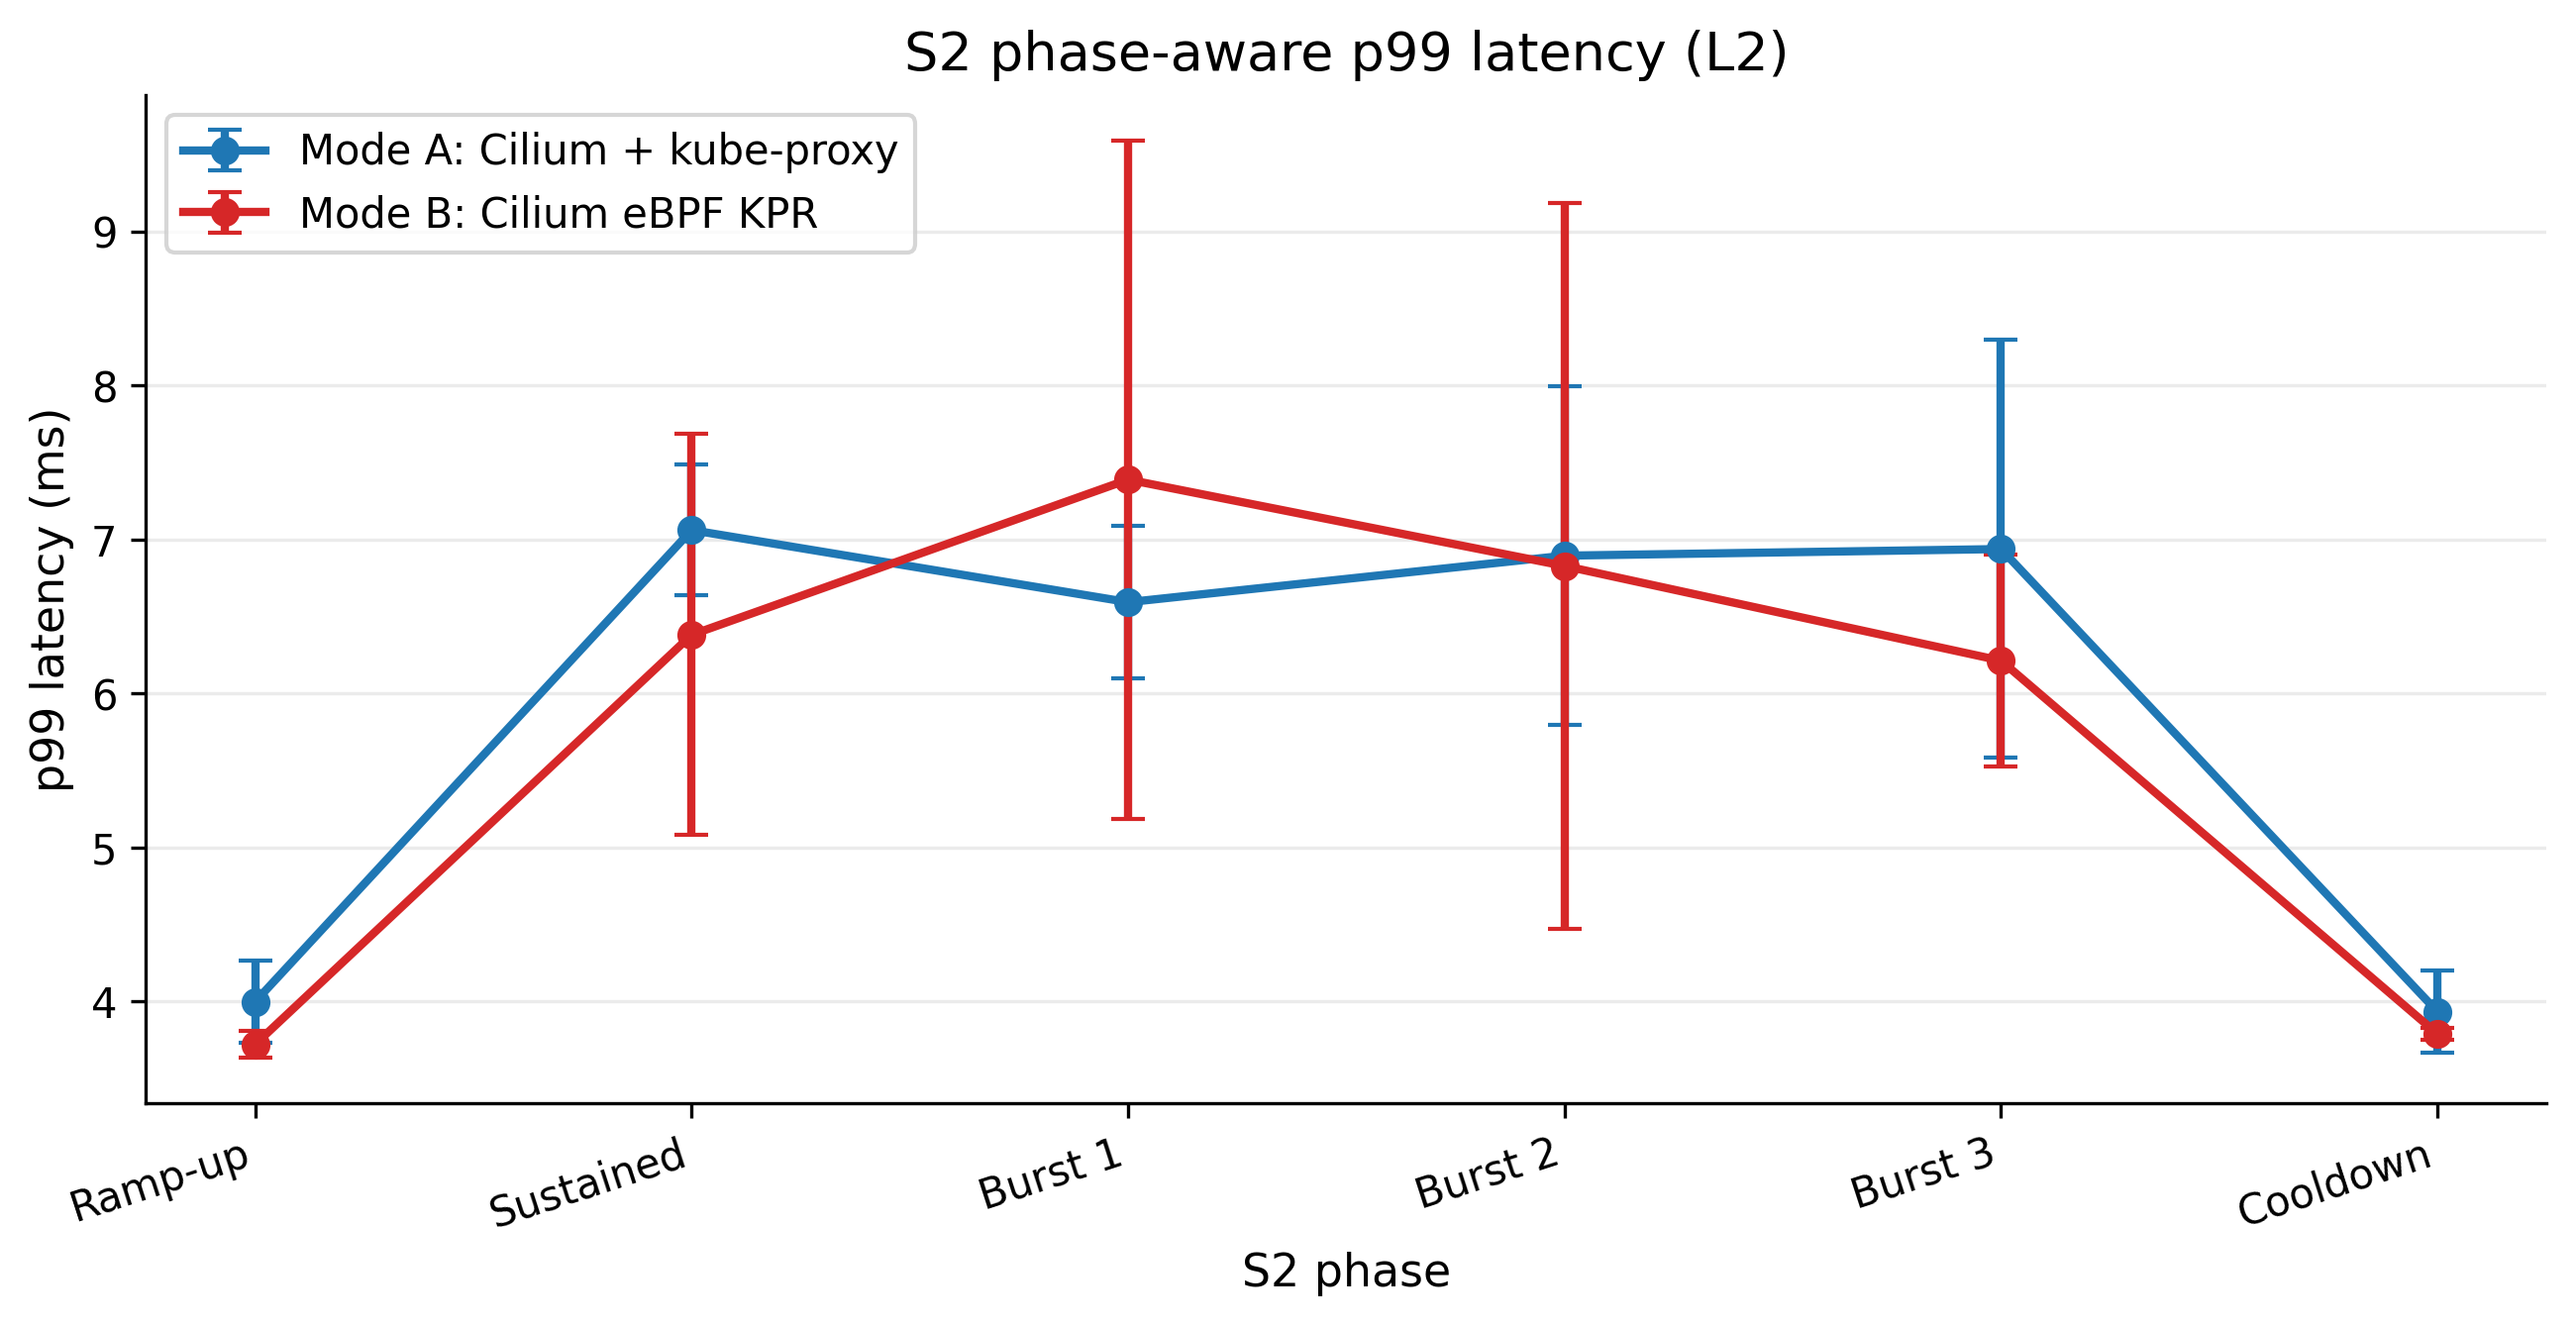
\includegraphics[width=0.90\textwidth]{../figures/thesis/fig-s2-phase-p99-l2.png}
    \caption{P99 latency theo pha trong S2 L2; các vạch dọc biểu diễn khoảng tin cậy 95\% quanh giá trị trung bình}
    \label{fig:s2-phase-p99-l2}
\end{figure}

\begin{table}[H]
\centering
\caption{So sánh p99 theo pha trong S2 L2}
\label{tab:s2-l2-p99-summary}
\small
\setlength{\tabcolsep}{4pt}
\renewcommand{\arraystretch}{1.2}
\begin{tabularx}{\textwidth}{>{\raggedright\arraybackslash}p{2.35cm}>{\raggedleft\arraybackslash}p{1.55cm}>{\raggedleft\arraybackslash}p{1.55cm}>{\raggedleft\arraybackslash}p{1.55cm}>{\raggedleft\arraybackslash}p{1.1cm}>{\raggedright\arraybackslash}X}
\toprule
\textbf{Pha} & \textbf{Mode A} & \textbf{Mode B} & \textbf{Delta} & \textbf{\(p\)} & \textbf{Diễn giải} \\
\midrule
Ramp-up & 3.998 ms & 3.721 ms & -6.934\% & 0.0367 & Significant \\
Sustained & 7.061 ms & 6.381 ms & -9.628\% & 0.1438 & Xu hướng \\
Burst 1 & 6.593 ms & 7.389 ms & +12.081\% & 0.2571 & Ngoại lệ, không significant \\
Burst 2 & 6.895 ms & 6.828 ms & -0.972\% & 0.9191 & Gần tương đương \\
Burst 3 & 6.938 ms & 6.213 ms & -10.445\% & 0.1339 & Xu hướng \\
Cooldown & 3.933 ms & 3.789 ms & -3.668\% & 0.1423 & Xu hướng nhẹ \\
\bottomrule
\end{tabularx}
\end{table}

\textbf{Phân tích.} Ở ramp-up, Mode B thấp hơn Mode A khoảng 6.9\% và đây là pha p99 duy nhất tại S2 L2 được đánh dấu significant. Sustained và Burst 3 cũng nghiêng về Mode B, nhưng chỉ nên xem là xu hướng. Ngoại lệ chính là Burst 1: Mode B cao hơn Mode A khoảng 12.1\%, dù chênh lệch này không significant. Burst 2 gần như tương đương.

Burst 1 là đợt tăng tải đột ngột đầu tiên sau sustained. Trong cửa sổ ngắn như vậy, một vài request chậm có thể kéo p99 lên rõ. Giá trị \(p=0.2571\) cho thấy chênh lệch này chưa đủ mạnh về mặt thống kê. Vì vậy, S2 L2 nên được đọc như vùng chuyển tiếp: Mode B tốt hơn ở một số pha, nhưng kết quả chưa đồng đều.

\textbf{Kết luận.} Với S2 L2, kết quả có lợi cho Mode B ở một số pha nhưng chưa đủ đồng đều để kết luận mạnh. Burst 1 là lời nhắc quan trọng rằng workload động cần được đọc theo phase, không nên gộp thành một nhận xét chung.

\subsection{S2 tại L3}

Hình~\ref{fig:s2-phase-p99-l3} trình bày S2 tại L3. Ở mức tải cao hơn, sustained và burst làm tail latency nhạy hơn. Khác với L2, Mode B có p99 trung bình thấp hơn Mode A ở tất cả các pha.

\begin{figure}[H]
    \centering
    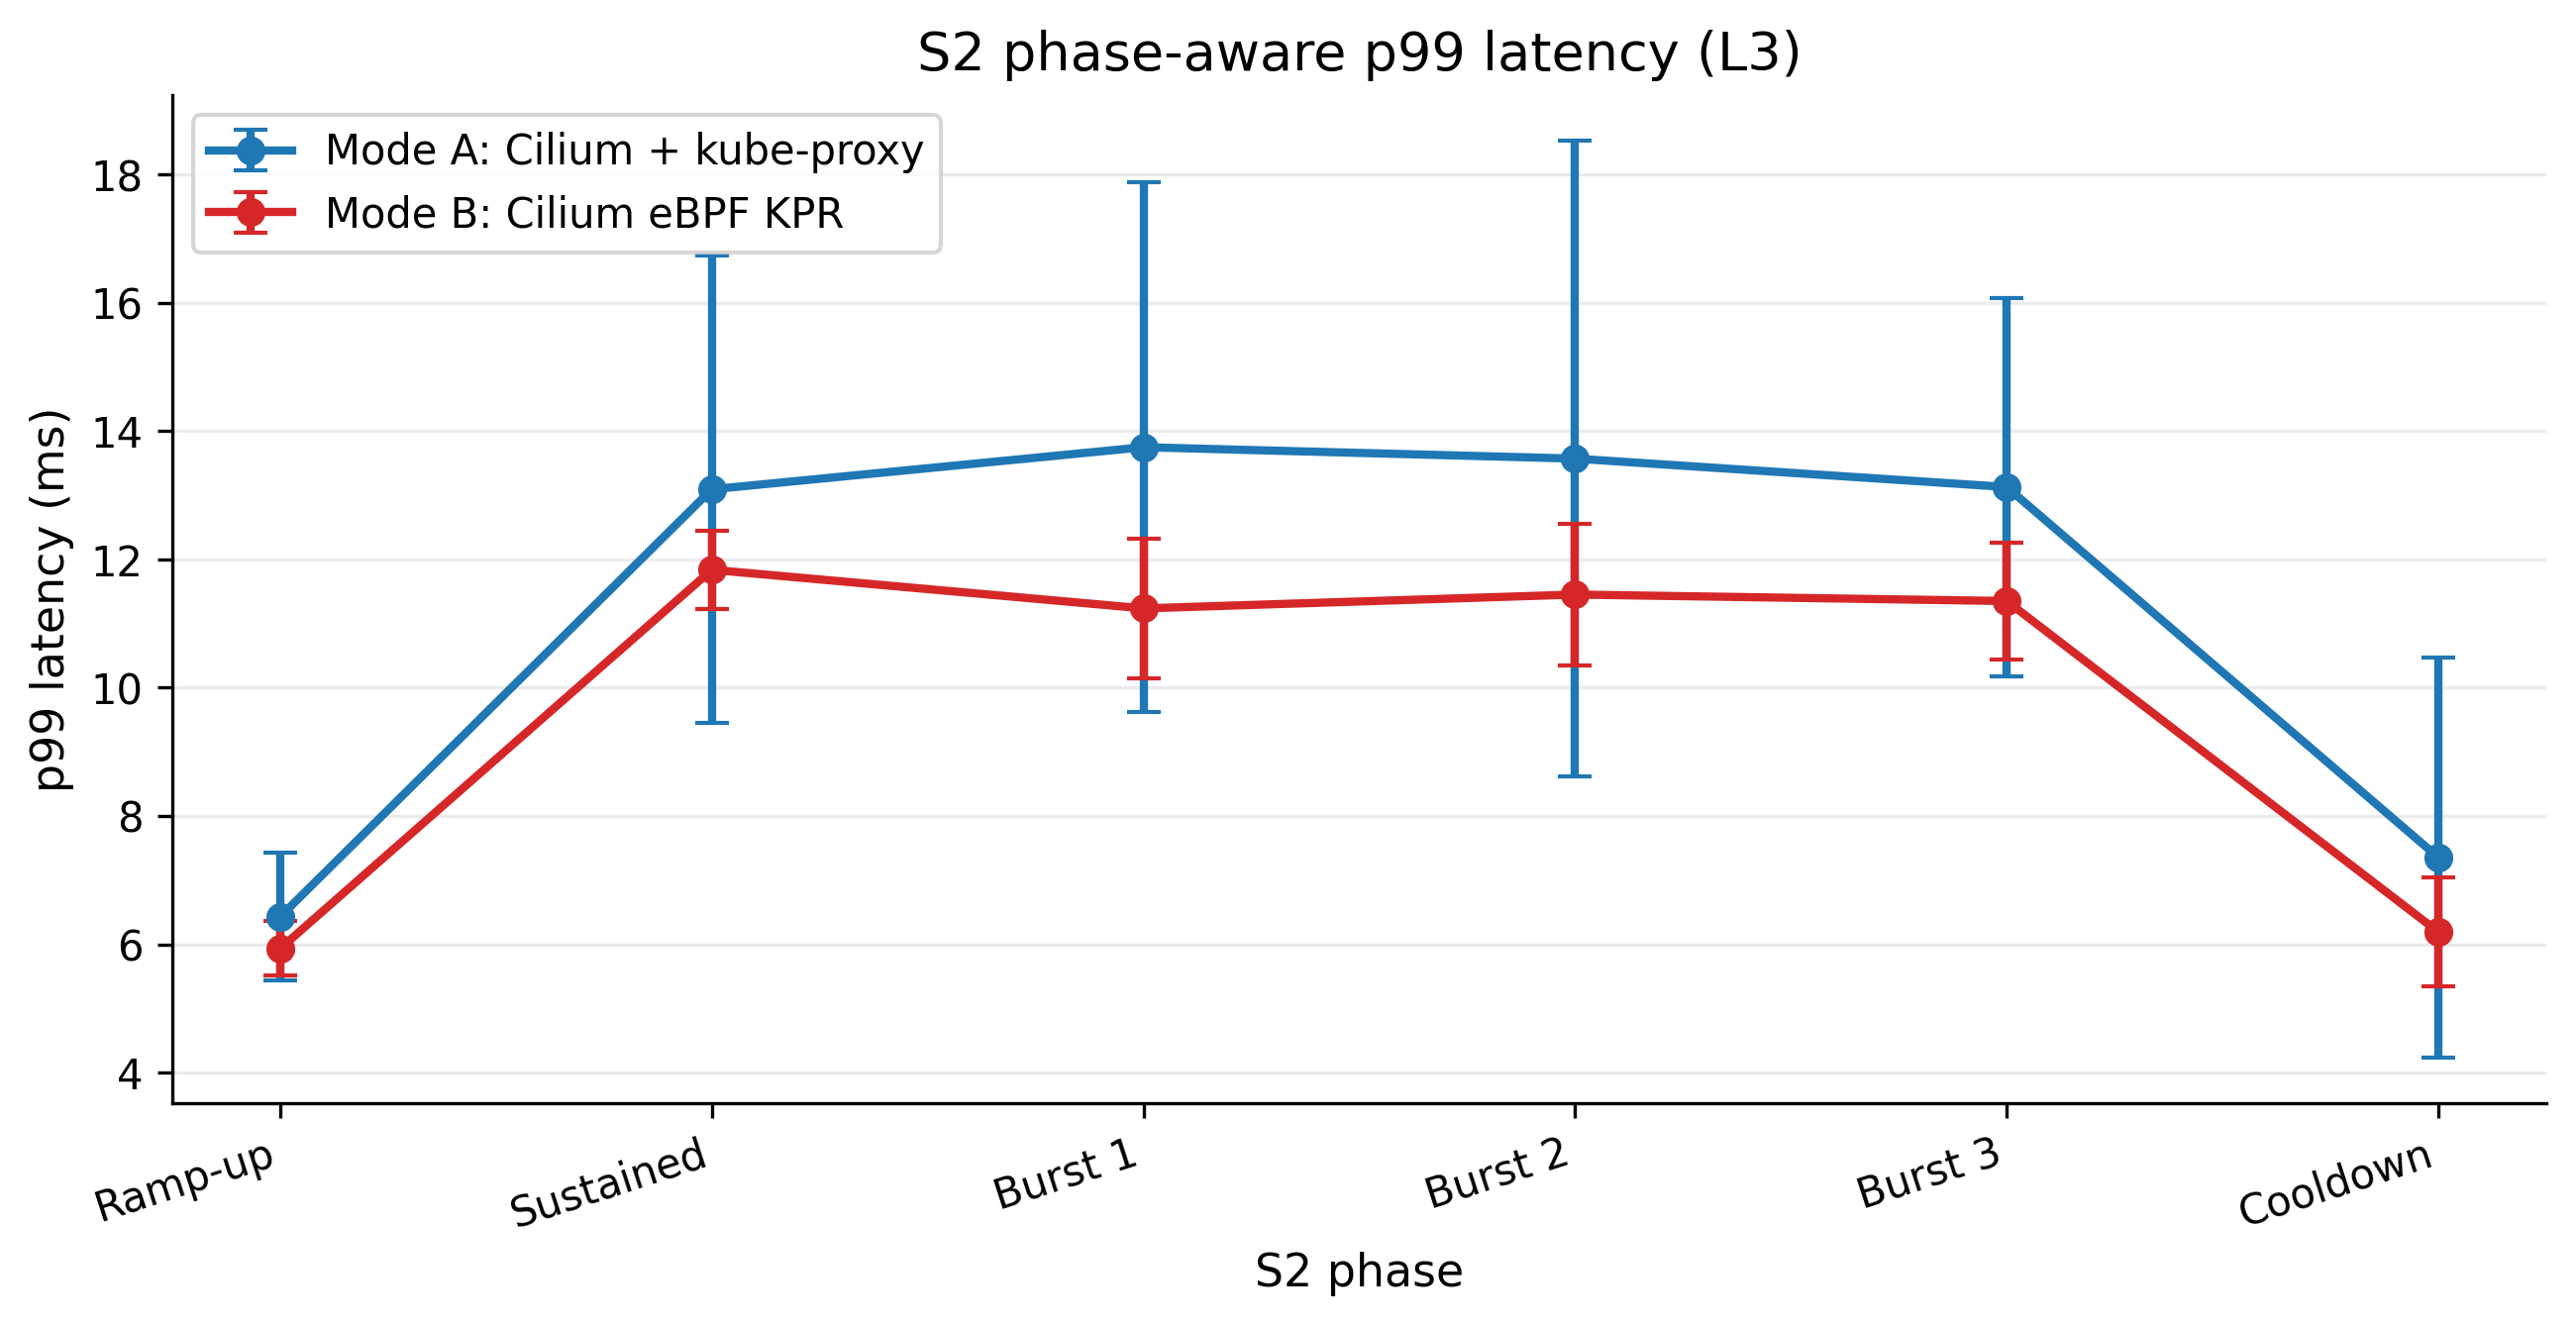
\includegraphics[width=0.90\textwidth]{../figures/thesis/fig-s2-phase-p99-l3.png}
    \caption{P99 latency theo pha trong S2 L3; các vạch dọc biểu diễn khoảng tin cậy 95\% quanh giá trị trung bình}
    \label{fig:s2-phase-p99-l3}
\end{figure}

\begin{table}[H]
\centering
\caption{So sánh p99 theo pha trong S2 L3}
\label{tab:s2-l3-p99-summary}
\small
\setlength{\tabcolsep}{4pt}
\renewcommand{\arraystretch}{1.2}
\begin{tabularx}{\textwidth}{>{\raggedright\arraybackslash}p{2.35cm}>{\raggedleft\arraybackslash}p{1.55cm}>{\raggedleft\arraybackslash}p{1.55cm}>{\raggedleft\arraybackslash}p{1.55cm}>{\raggedleft\arraybackslash}p{1.1cm}>{\raggedright\arraybackslash}X}
\toprule
\textbf{Pha} & \textbf{Mode A} & \textbf{Mode B} & \textbf{Delta} & \textbf{\(p\)} & \textbf{Diễn giải} \\
\midrule
Ramp-up & 6.431 ms & 5.934 ms & -7.724\% & 0.1531 & Xu hướng \\
Sustained & 13.094 ms & 11.839 ms & -9.587\% & 0.2751 & Xu hướng \\
Burst 1 & 13.750 ms & 11.237 ms & -18.271\% & 0.1119 & Xu hướng mạnh \\
Burst 2 & 13.572 ms & 11.453 ms & -15.618\% & 0.2029 & Xu hướng mạnh \\
Burst 3 & 13.129 ms & 11.352 ms & -13.532\% & 0.1116 & Xu hướng \\
Cooldown & 7.355 ms & 6.193 ms & -15.800\% & 0.2466 & Xu hướng \\
\bottomrule
\end{tabularx}
\end{table}

\textbf{Phân tích.} Ở L3, toàn bộ delta p99 đều âm. Các pha burst có chênh lệch lớn hơn: Burst 1 khoảng -18.3\%, Burst 2 khoảng -15.6\% và Burst 3 khoảng -13.5\%. Đây là mức chênh đáng chú ý vì xuất hiện ở tải cao, đúng nơi tail latency dễ bộc lộ nhất.

Điểm cần thận trọng là các dòng p99 L3 chưa significant. Vạch CI của Mode A dài hơn Mode B ở nhiều pha, đặc biệt sustained và burst, cho thấy p99 của Mode A dao động nhiều hơn giữa ba lần chạy. Vì các \(p\)-value vẫn lớn hơn 0.05, kết luận phù hợp là Mode B có xu hướng p99 thấp hơn và ổn định hơn trong tập run hiện tại, nhưng chưa đủ để khẳng định chắc chắn cho từng pha.

Về cơ chế, L3 đặt datapath vào vùng nhạy với tail latency hơn. Khi tải nền cao và burst xuất hiện, queueing, trạng thái kết nối và scheduling jitter dễ tích lũy vào p99. Mẫu hình toàn delta âm phù hợp với giả thuyết Mode B có lợi thế ở tải cao, nhưng vẫn chịu giới hạn bởi variance và số lần lặp nhỏ.

\textbf{Kết luận.} S2 L3 là phần ủng hộ rõ nhất cho nhận định rằng Mode B có thể có lợi thế tail latency trong workload động ở tải cao. Dù vậy, vì chưa significant ở từng pha, cách viết phù hợp là ``xu hướng mạnh'' thay vì khẳng định tuyệt đối.

\subsection{Vai trò của heatmap S2}

Hình~\ref{fig:s2-p99-delta-heatmap} tóm tắt chênh lệch p99 của Mode B so với Mode A theo pha và mức tải. Giá trị âm nghĩa là Mode B thấp hơn; giá trị dương nghĩa là Mode B cao hơn.

\begin{figure}[H]
    \centering
    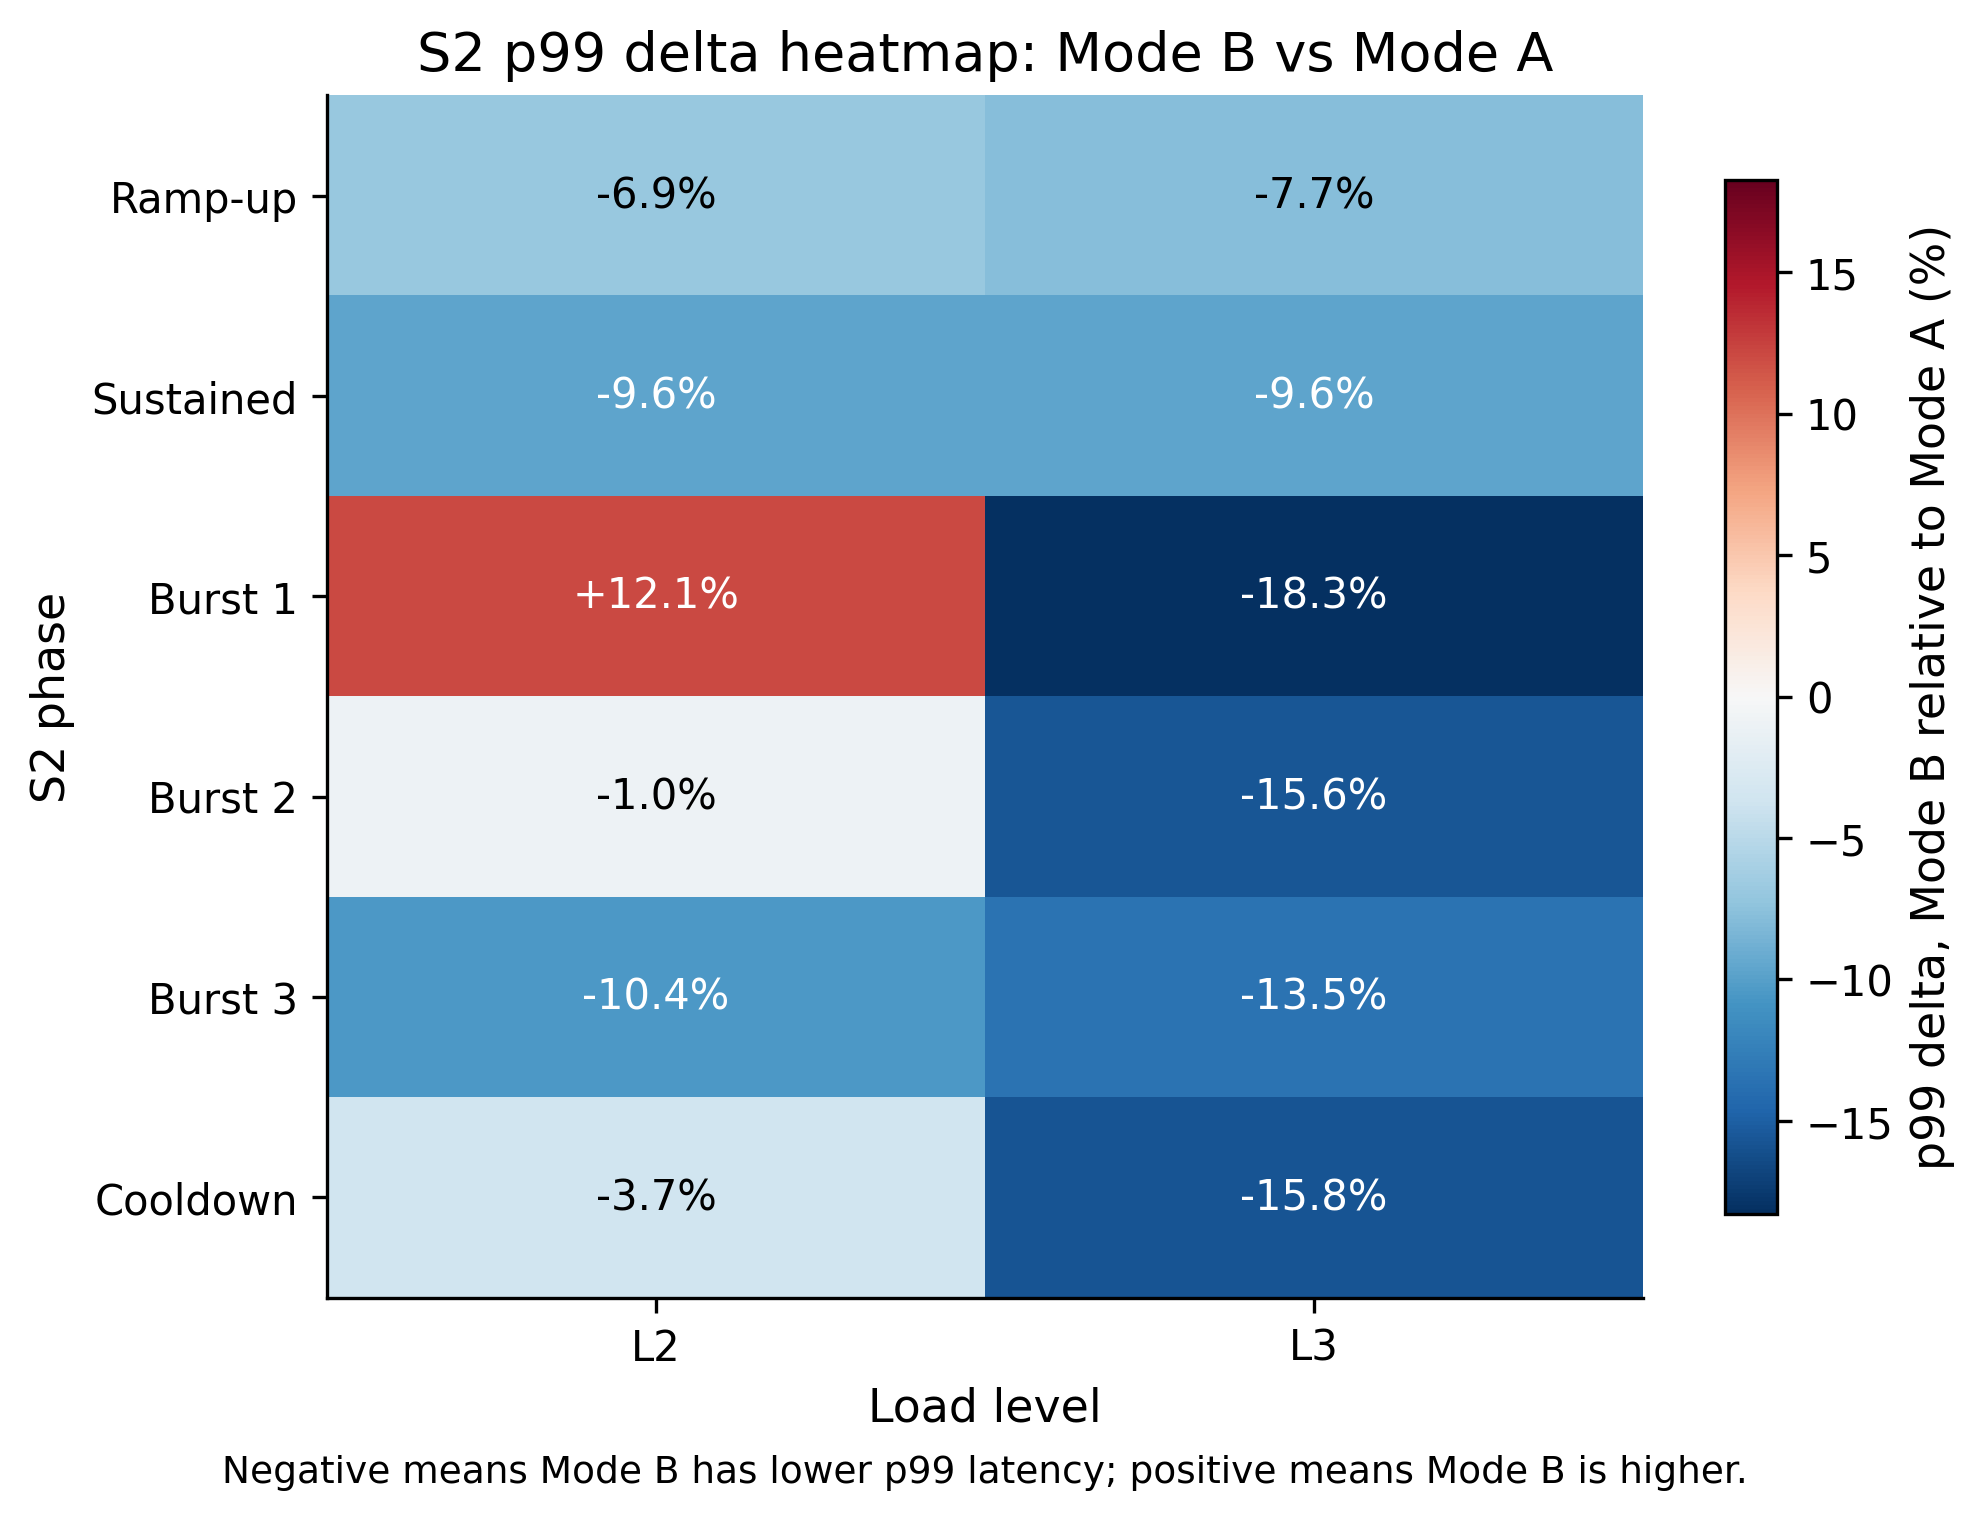
\includegraphics[width=0.78\textwidth]{../figures/thesis/fig-s2-p99-delta-heatmap.png}
    \caption{Heatmap chênh lệch p99 trong S2 theo pha và mức tải}
    \label{fig:s2-p99-delta-heatmap}
\end{figure}

\textbf{Phân tích.} Heatmap cho thấy hai điểm chính: L3 có delta âm ở toàn bộ pha, còn L2 có ngoại lệ Burst 1 dương. Hình này giúp nhận diện nhanh mẫu hình theo pha, nhưng chỉ thể hiện chênh lệch trung bình. Vì vậy, diễn giải chính vẫn phải dựa vào biểu đồ p99 theo pha, CI, \(p\)-value và độ biến động.

Hình~\ref{fig:s2-grafana-cpu-evidence} và Hình~\ref{fig:s2-grafana-memory-evidence} bổ sung bối cảnh vận hành cho S2 L3. Hai hình kiểm tra CPU và memory của namespace benchmark ở mức tải stress cao hơn.

Trong cửa sổ S2 L3 được lưu, không thấy dấu hiệu CPU hoặc memory pressure nghiêm trọng. Tuy nhiên, ảnh Grafana không được căn chỉnh chính xác theo từng pha, nên chỉ dùng như sanity check, không dùng để quy kết spike p99 cho CPU/memory. Các ảnh S2 L2 và bản phóng lớn được đặt ở Phụ lục~E.

\begin{figure}[H]
    \centering
    \textbf{Mode A -- CPU namespace}\\[0.25em]
    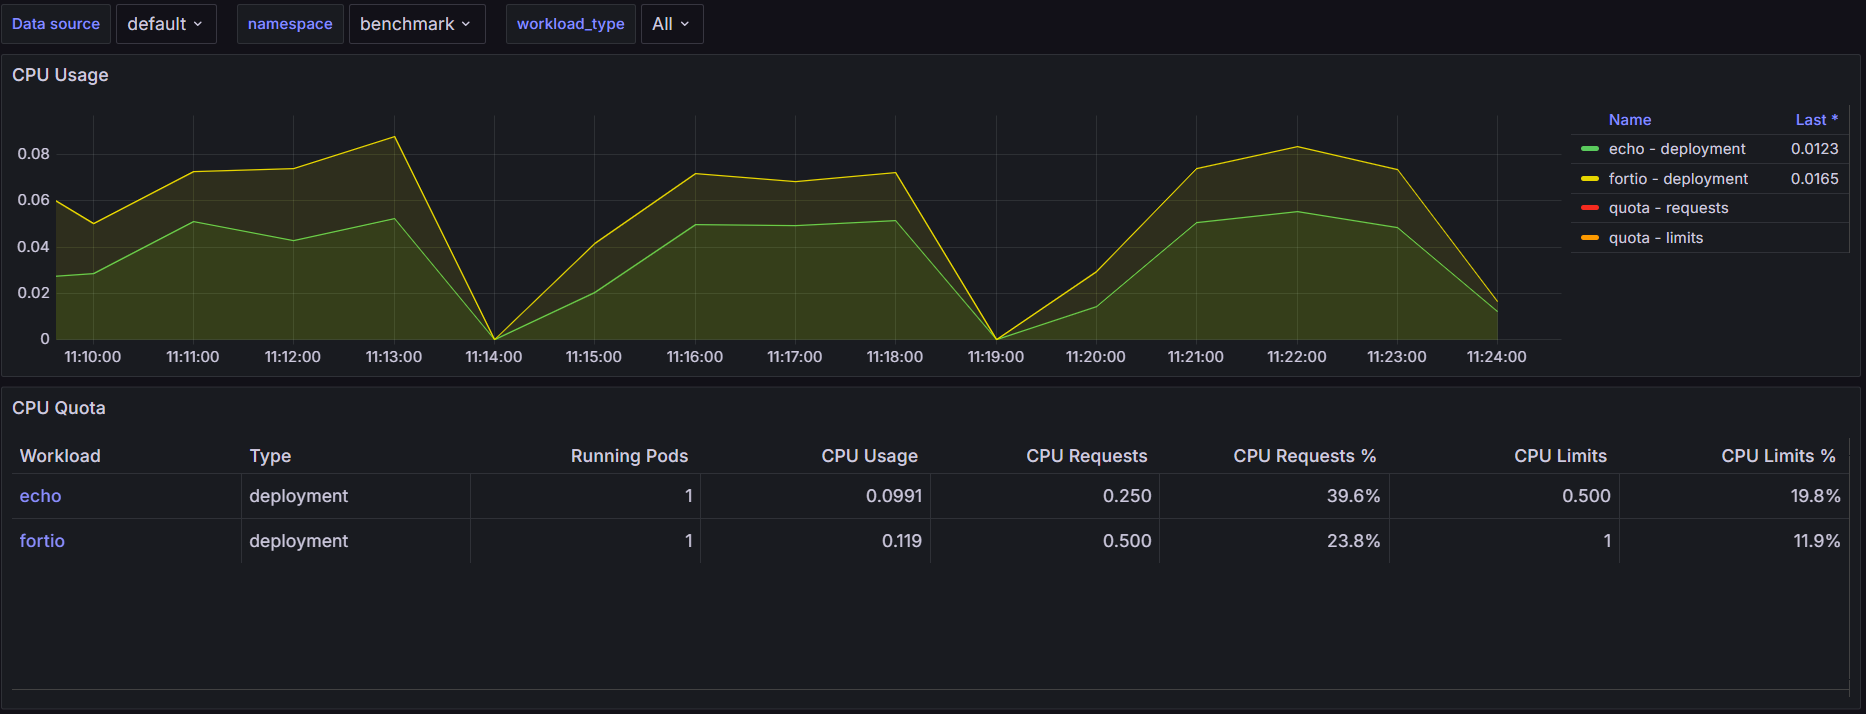
\includegraphics[width=0.88\textwidth]{../figures/grafana/modeA/grafana-ns-cpu-S2-L3-R1.png}
    \vspace{0.5em}
    
    \textbf{Mode B -- CPU namespace}\\[0.25em]
    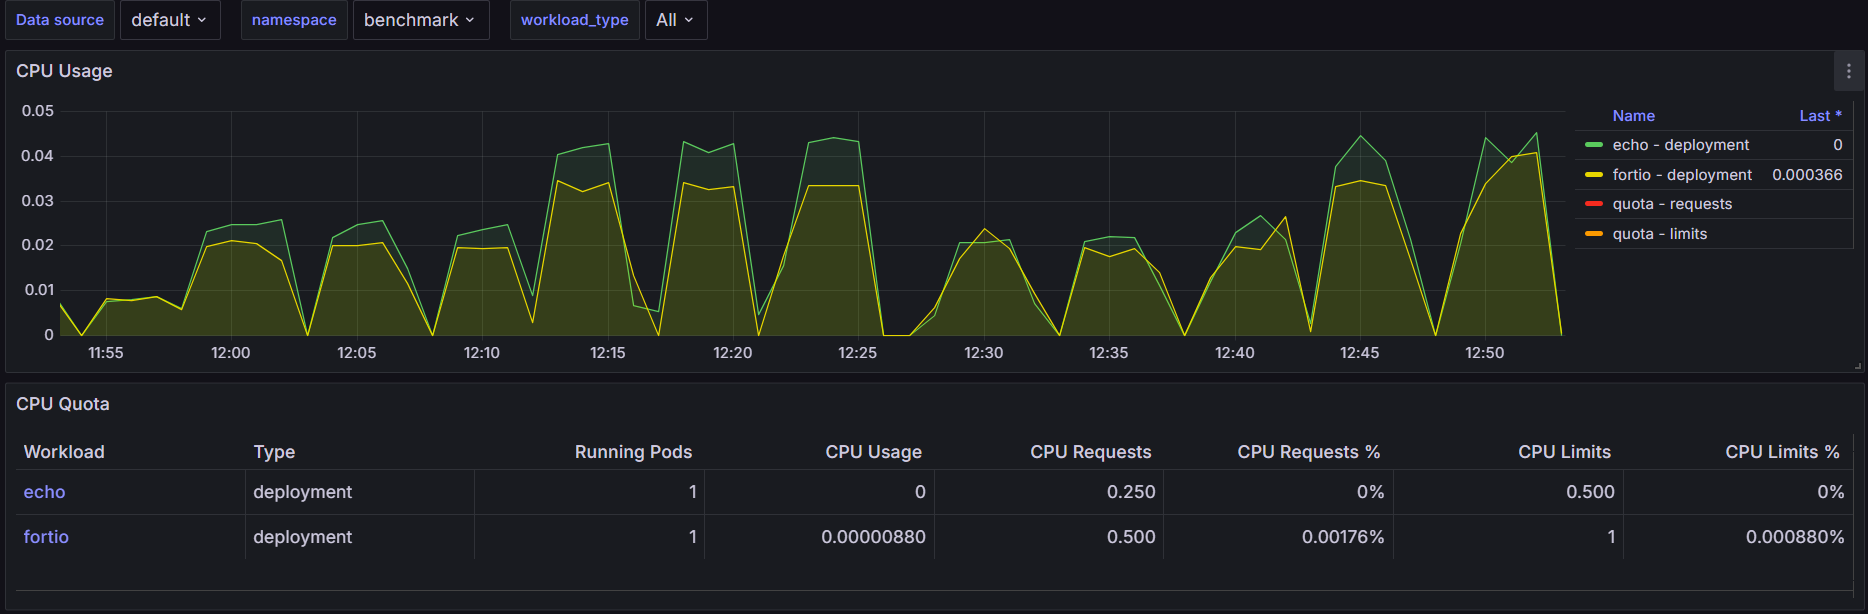
\includegraphics[width=0.88\textwidth]{../figures/grafana/modeB/grafana-ns-cpu-S2-L3.png}
    \caption{Bằng chứng Grafana namespace-level về CPU cho S2 L3 ở Mode A và Mode B; ảnh dùng như sanity check về resource pressure, không thay thế phân tích p99 theo pha}
    \label{fig:s2-grafana-cpu-evidence}
\end{figure}

\begin{figure}[H]
    \centering
    \textbf{Mode A -- memory namespace}\\[0.25em]
    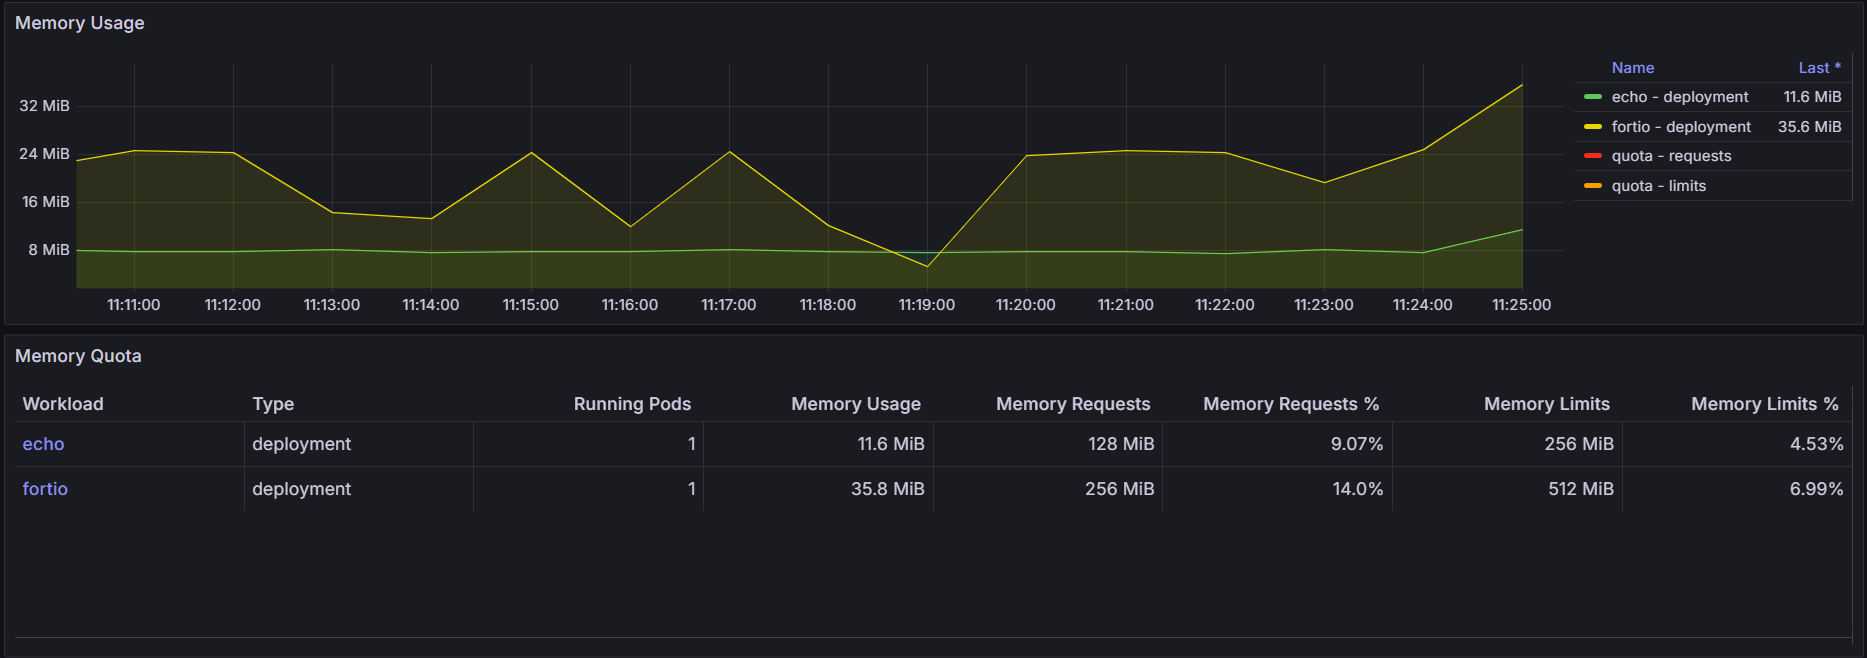
\includegraphics[width=0.88\textwidth]{../figures/grafana/modeA/grafana-ns-mem-S2-L3-R1.png}
    \vspace{0.5em}

    \textbf{Mode B -- memory namespace}\\[0.25em]
    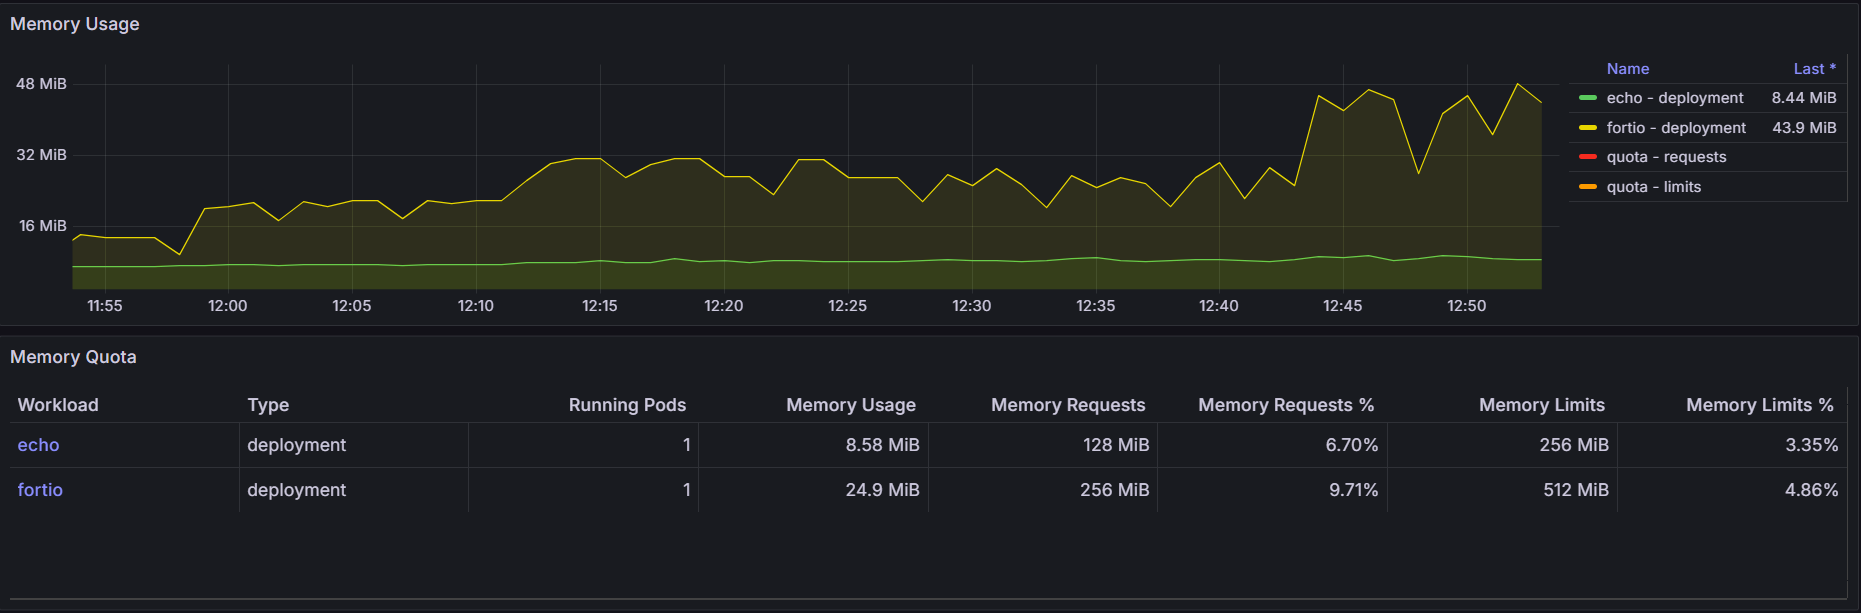
\includegraphics[width=0.88\textwidth]{../figures/grafana/modeB/grafana-ns-mem-S2-L3.png}
    \caption{Bằng chứng Grafana namespace-level về memory cho S2 L3 ở Mode A và Mode B; ảnh dùng như sanity check về resource pressure, không thay thế phân tích p99 theo pha}
    \label{fig:s2-grafana-memory-evidence}
\end{figure}

\textbf{Kết luận.} Với S2, kết luận an toàn là Mode B có xu hướng p99 tốt hơn rõ hơn ở L3, trong khi L2 vẫn có tính pha trộn. Kết quả này hỗ trợ nhận định về lợi thế datapath dưới tải cao và workload động, nhưng không đủ để khẳng định tuyệt đối cho mọi pha.

\section{Kết quả S3: chi phí NetworkPolicy}

S3 kiểm tra chi phí khi bật NetworkPolicy trong Mode B. Đây không phải là so sánh Mode A với Mode B; biến duy nhất được thay đổi là trạng thái policy OFF/ON trong cùng Mode B. Mục tiêu là xem một chính sách đơn giản có làm tăng p99 latency hoặc làm giảm achieved RPS đáng kể hay không.

Hai biểu đồ chính của S3 là p99 và achieved RPS khi policy OFF/ON. P99 cho biết tác động lên tail latency; RPS kiểm tra hai trạng thái vẫn được đo ở mức tải tương đương.

\begin{figure}[H]
    \centering
    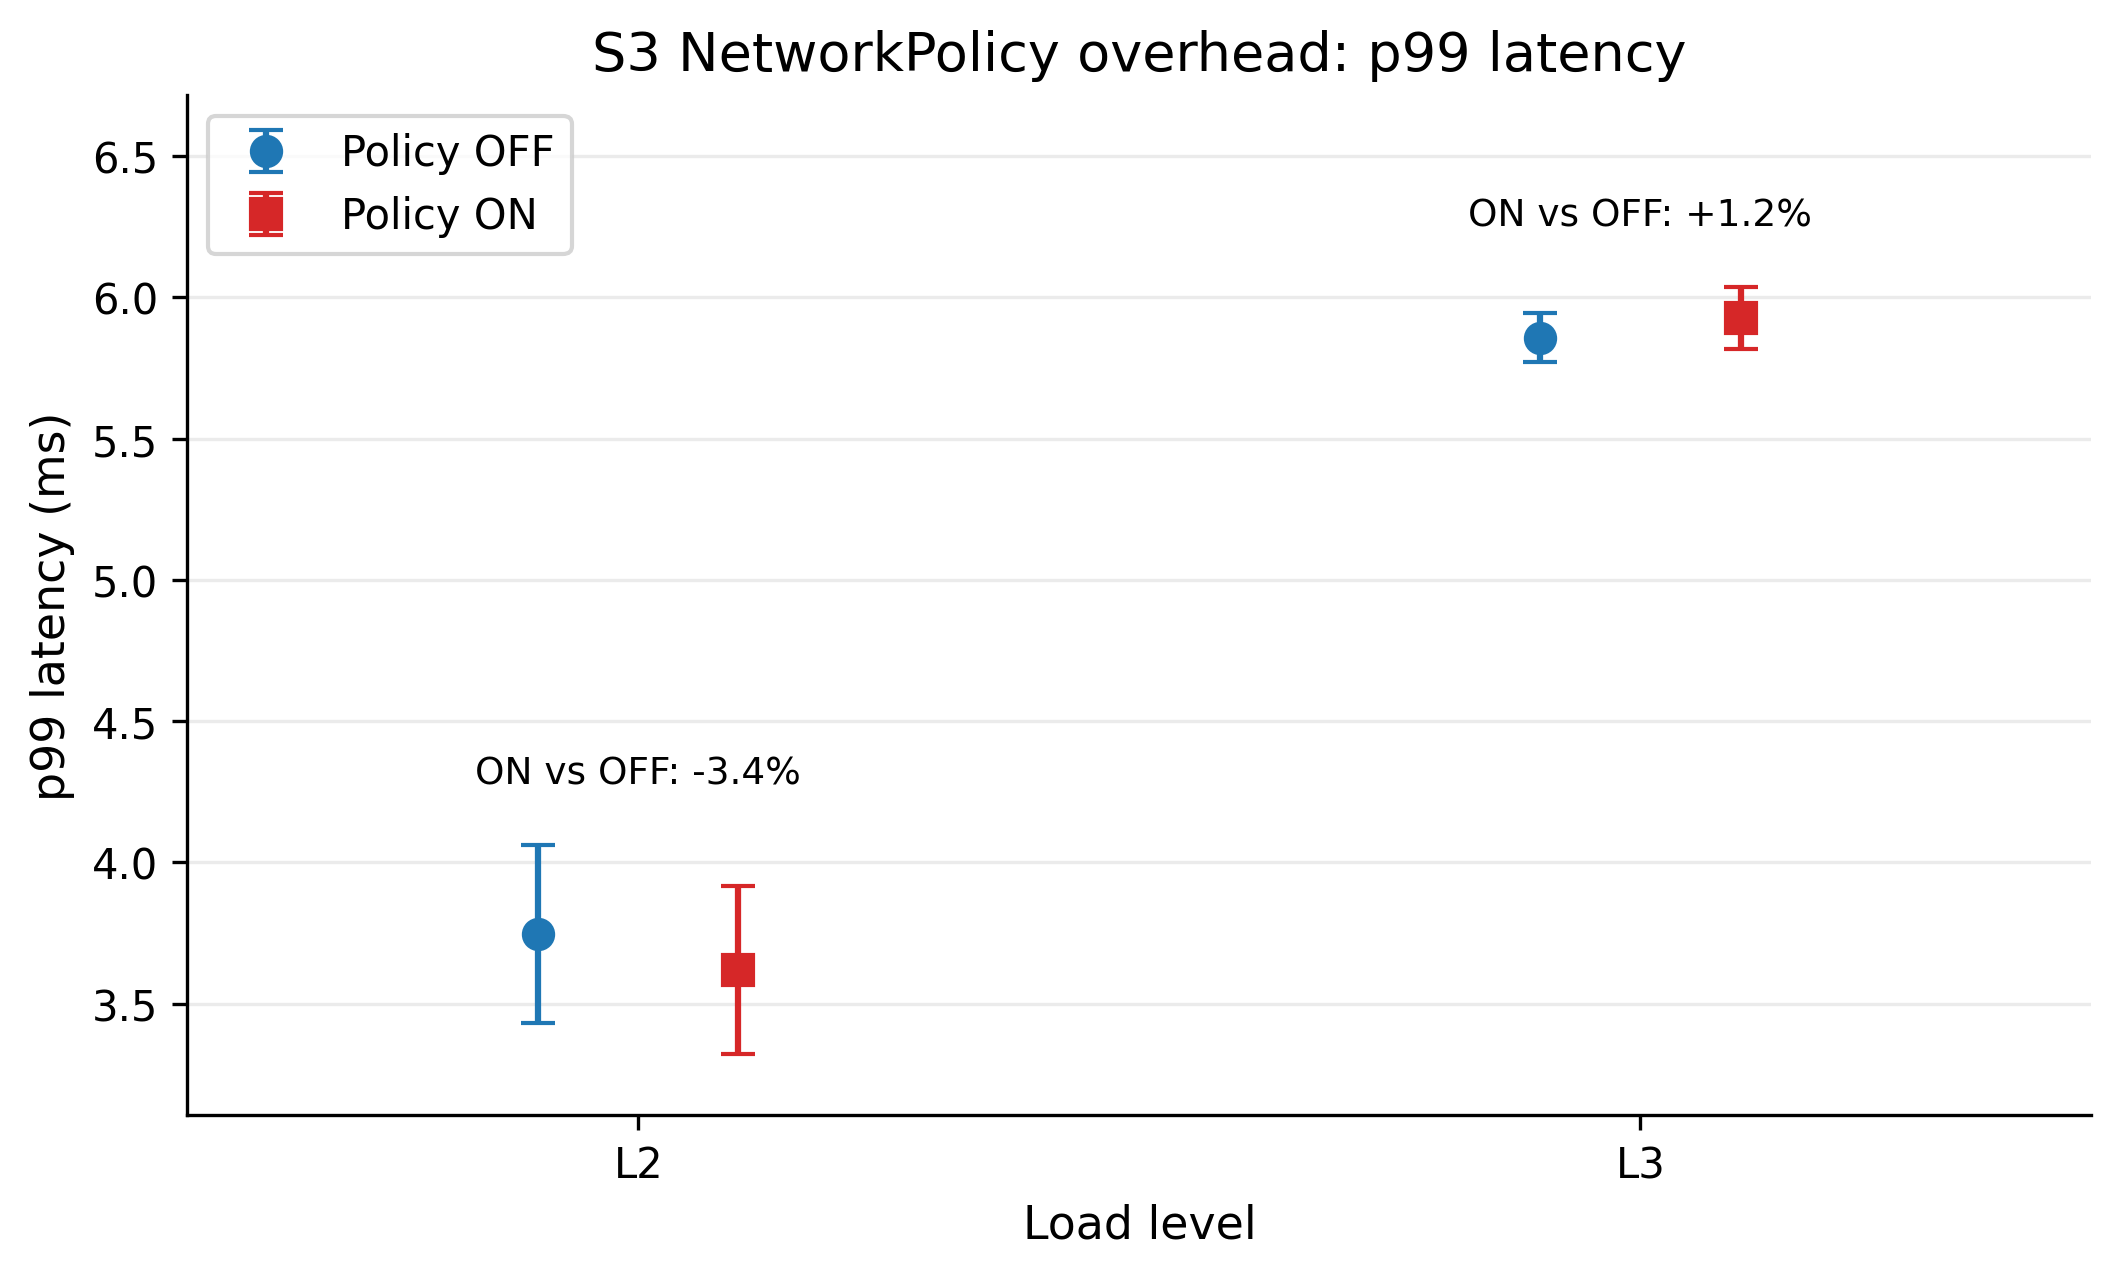
\includegraphics[width=0.82\textwidth]{../figures/thesis/fig-s3-policy-overhead-p99.png}
    \caption{P99 latency của S3 khi chính sách OFF và ON trong Mode B; các vạch dọc biểu diễn khoảng tin cậy 95\% quanh giá trị trung bình}
    \label{fig:s3-policy-overhead-p99}
\end{figure}

\begin{table}[H]
\centering
\caption{Tóm tắt kết quả S3 chính sách OFF và ON}
\label{tab:s3-policy-summary}
\renewcommand{\arraystretch}{1.2}
\begin{tabularx}{\textwidth}{>{\raggedright\arraybackslash}p{1.1cm}>{\raggedright\arraybackslash}p{1.4cm}>{\raggedleft\arraybackslash}p{1.8cm}>{\raggedleft\arraybackslash}p{3.0cm}>{\raggedleft\arraybackslash}p{1.9cm}>{\raggedleft\arraybackslash}X}
\toprule
\textbf{Tải} & \textbf{Policy} & \textbf{p99 mean} & \textbf{CI 95\%} & \textbf{RPS mean} & \textbf{Lỗi} \\
\midrule
L2 & OFF & 3.747 ms & 3.431--4.063 ms & 399.992 & 0.0\% \\
L2 & ON & 3.619 ms & 3.323--3.916 ms & 399.992 & 0.0\% \\
L3 & OFF & 5.857 ms & 5.770--5.944 ms & 799.974 & 0.0\% \\
L3 & ON & 5.928 ms & 5.818--6.037 ms & 799.965 & 0.0\% \\
\bottomrule
\end{tabularx}
\end{table}

\textbf{Phân tích.} Kết quả p99 cho thấy OFF và ON rất gần nhau. Ở L2, ON thấp hơn OFF một lượng nhỏ, nhưng không nên hiểu rằng policy làm tăng hiệu năng. Ở L3, ON cao hơn OFF khoảng 0.071 ms, tương đương khoảng 1.2\%; đây là mức chênh nhỏ về mặt thực tế. Các vạch CI 95\% cũng gần nhau, nên không có cơ sở để kết luận overhead p99 lớn trong dataset hiện tại.

\begin{figure}[H]
    \centering
    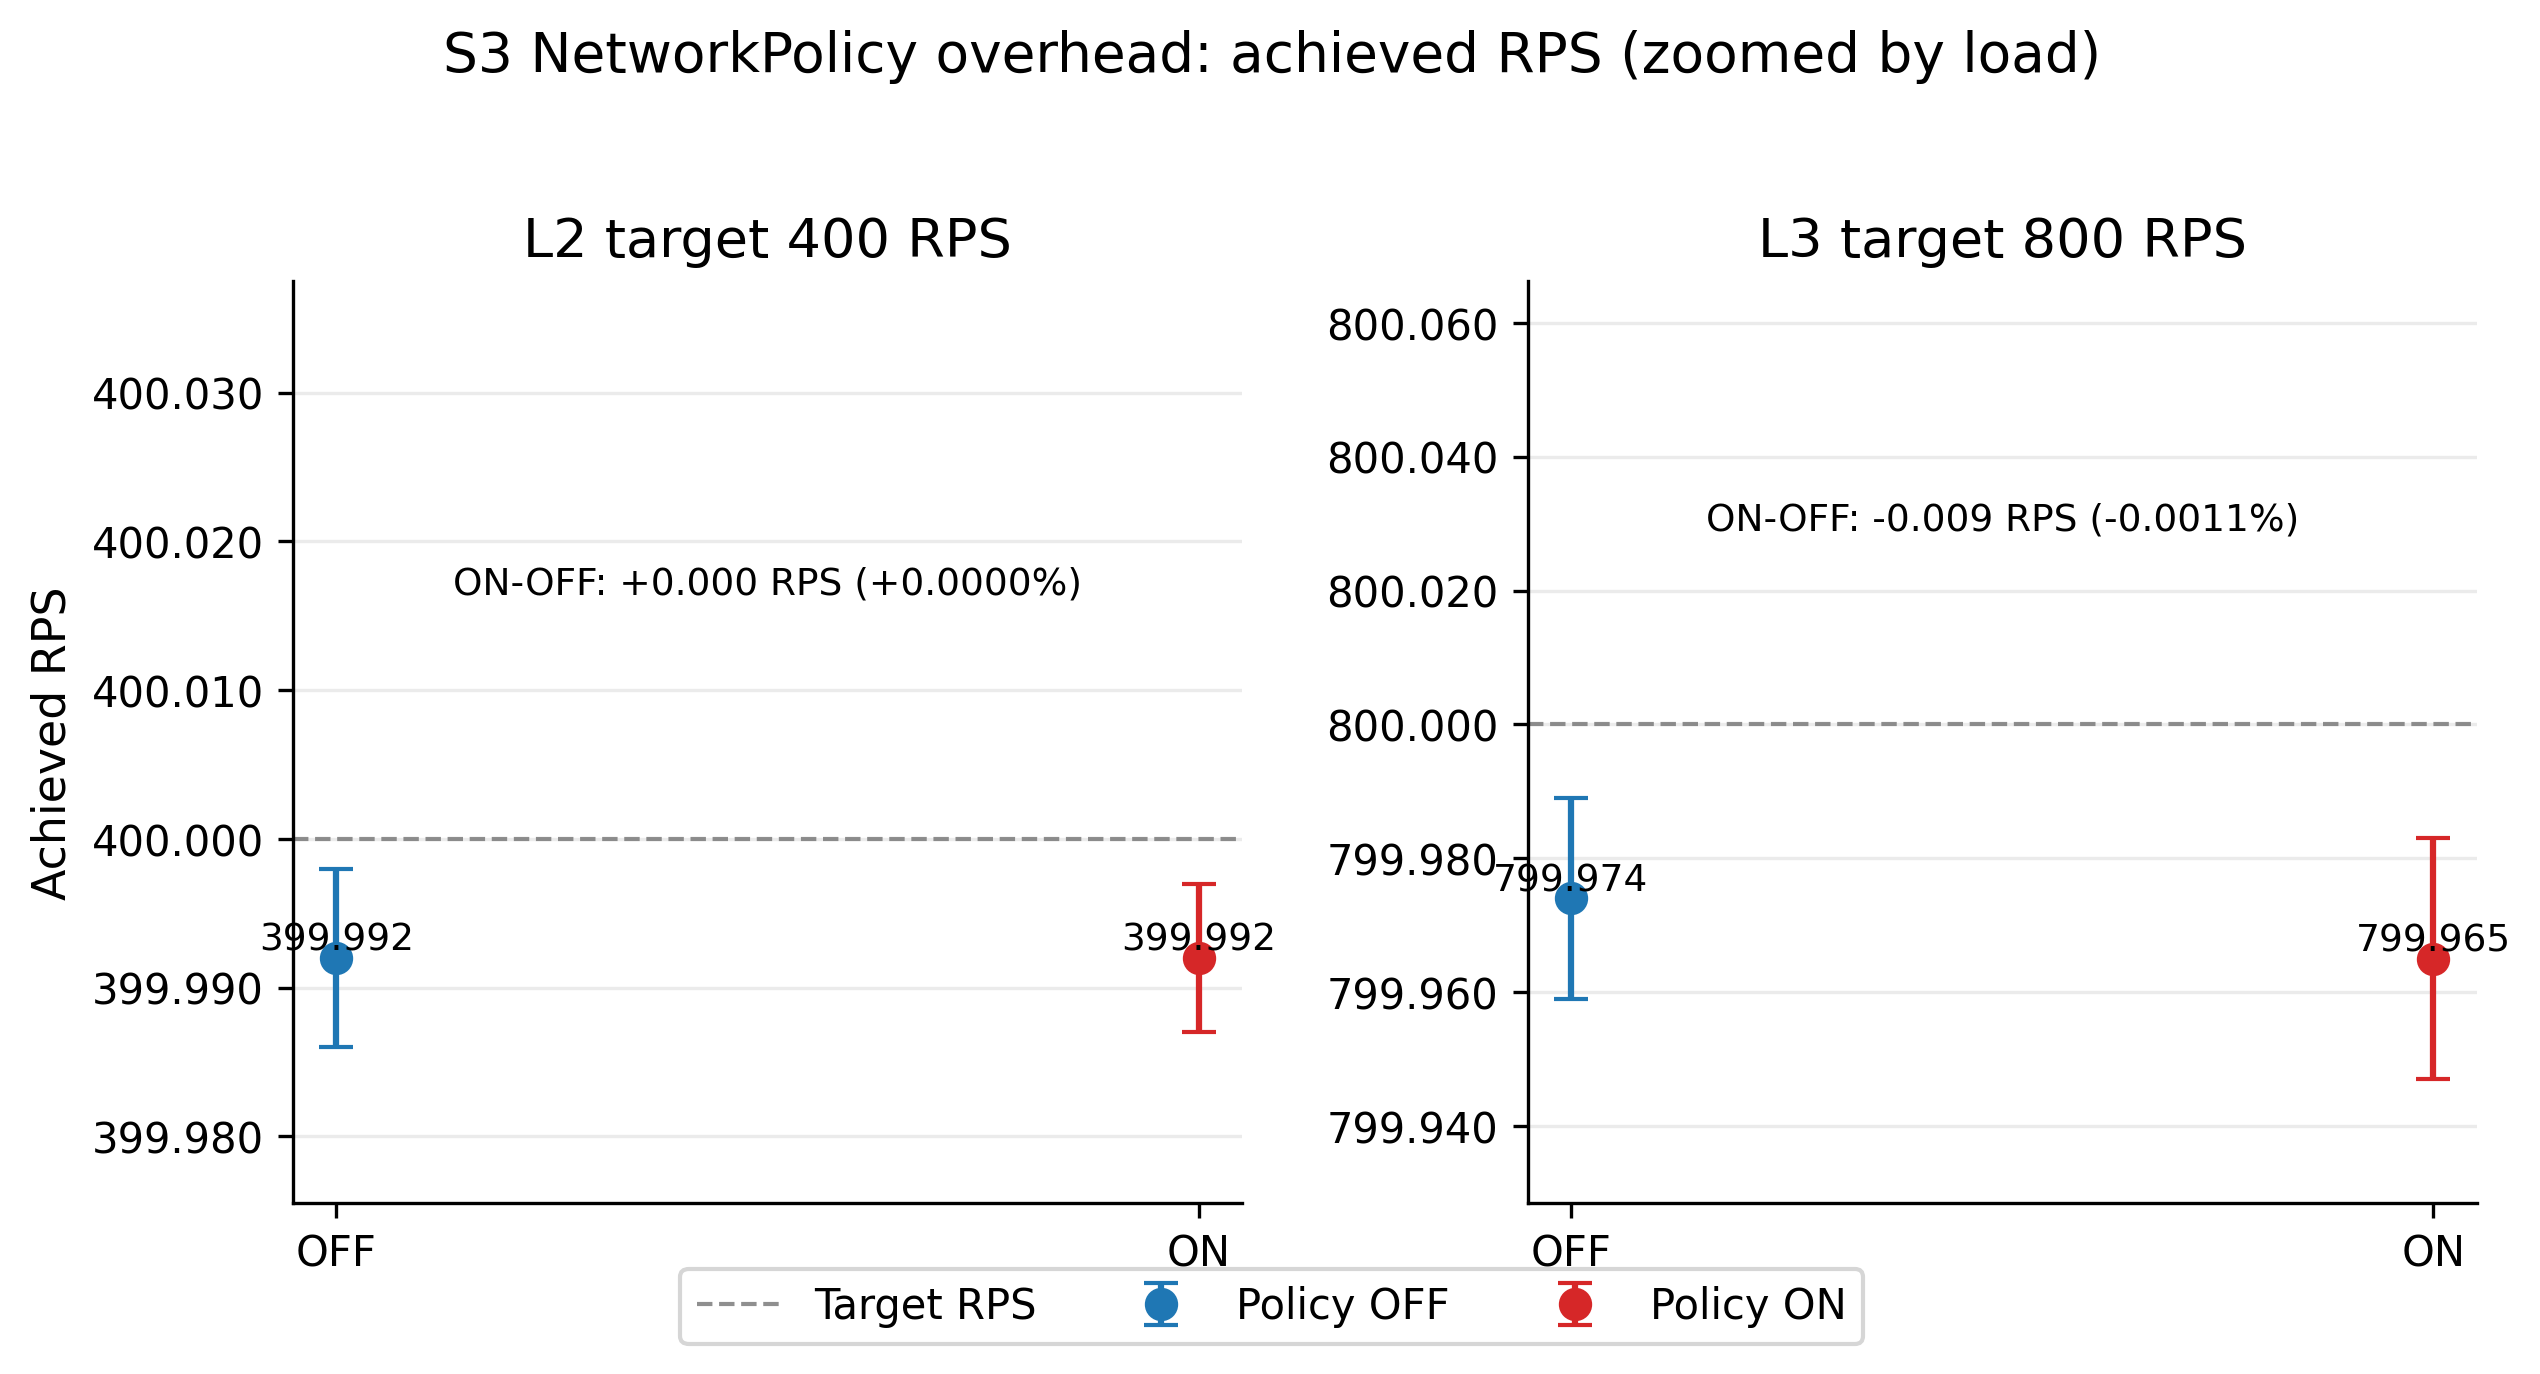
\includegraphics[width=0.82\textwidth]{../figures/thesis/fig-s3-policy-overhead-rps.png}
    \caption{RPS đạt được của S3 khi chính sách OFF và ON trong Mode B; các vạch dọc biểu diễn khoảng tin cậy 95\% quanh giá trị trung bình}
    \label{fig:s3-policy-overhead-rps}
\end{figure}

Hình~\ref{fig:s3-policy-overhead-rps} cho thấy achieved RPS gần như không đổi giữa OFF và ON, còn error rate bằng 0\%. Khi đọc cùng p99, cách diễn giải phù hợp là overhead quan sát được nhỏ. Tuy nhiên, error rate bằng 0\% chỉ nói rằng request hoàn tất thành công; nó không chứng minh policy enforcement không có chi phí.

Về cơ chế, kết quả OFF/ON gần nhau là hợp lý với policy đơn giản, số endpoint nhỏ và traffic benchmark đều được cho phép. Hình~\ref{fig:s3-hubble-policy-evidence} bổ sung bằng chứng Hubble ở mức flow/verdict: forward-case cho thấy flow được \texttt{forwarded}, còn deny-case thủ công minh họa verdict \texttt{Policy denied}.

Hubble chỉ là evidence bổ trợ về policy enforcement và observability. Kết luận overhead vẫn dựa trên p99, RPS và error rate từ Fortio. Các ảnh Hubble phụ khác được đặt ở Phụ lục~E.

\begin{figure}[H]
    \centering
    \textbf{Forward-case trong namespace benchmark}\\[0.25em]
    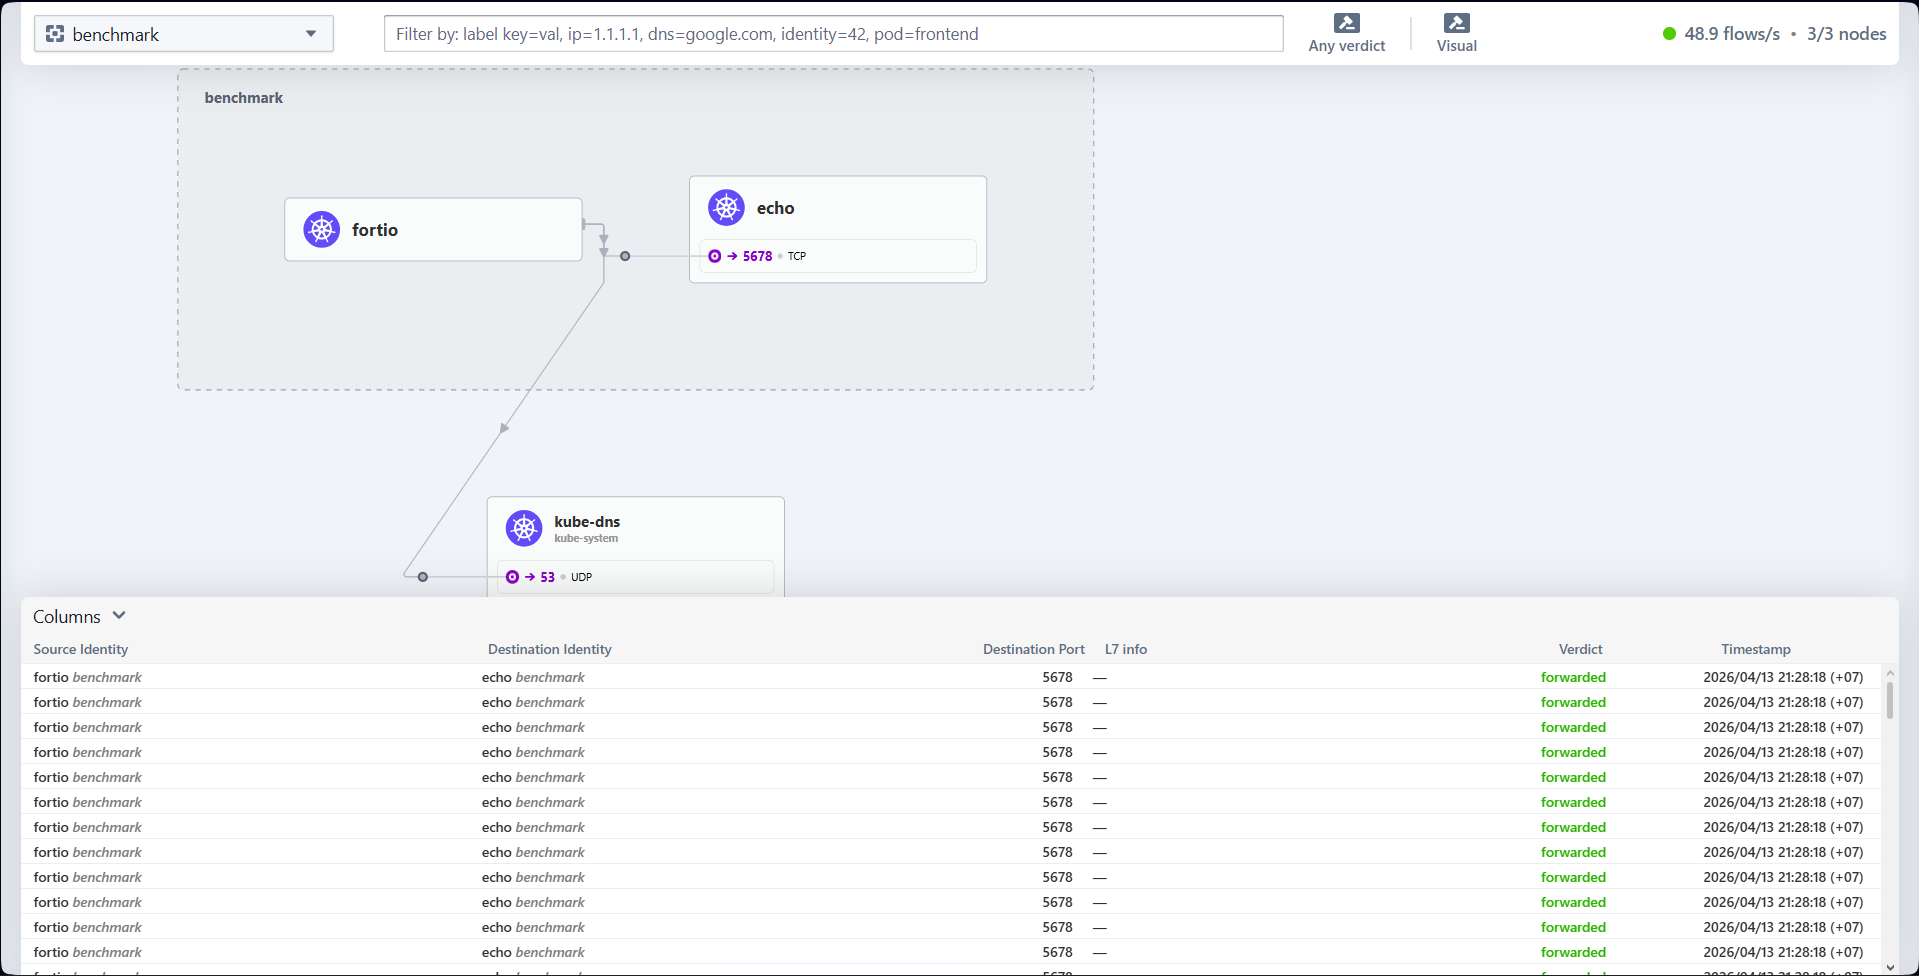
\includegraphics[width=0.86\textwidth]{../figures/hubble/fig-13b-hubble-forwarded-case.png}
    \vspace{0.4em}
    
    \textbf{Manual deny-case với Policy denied}\\[0.25em]
    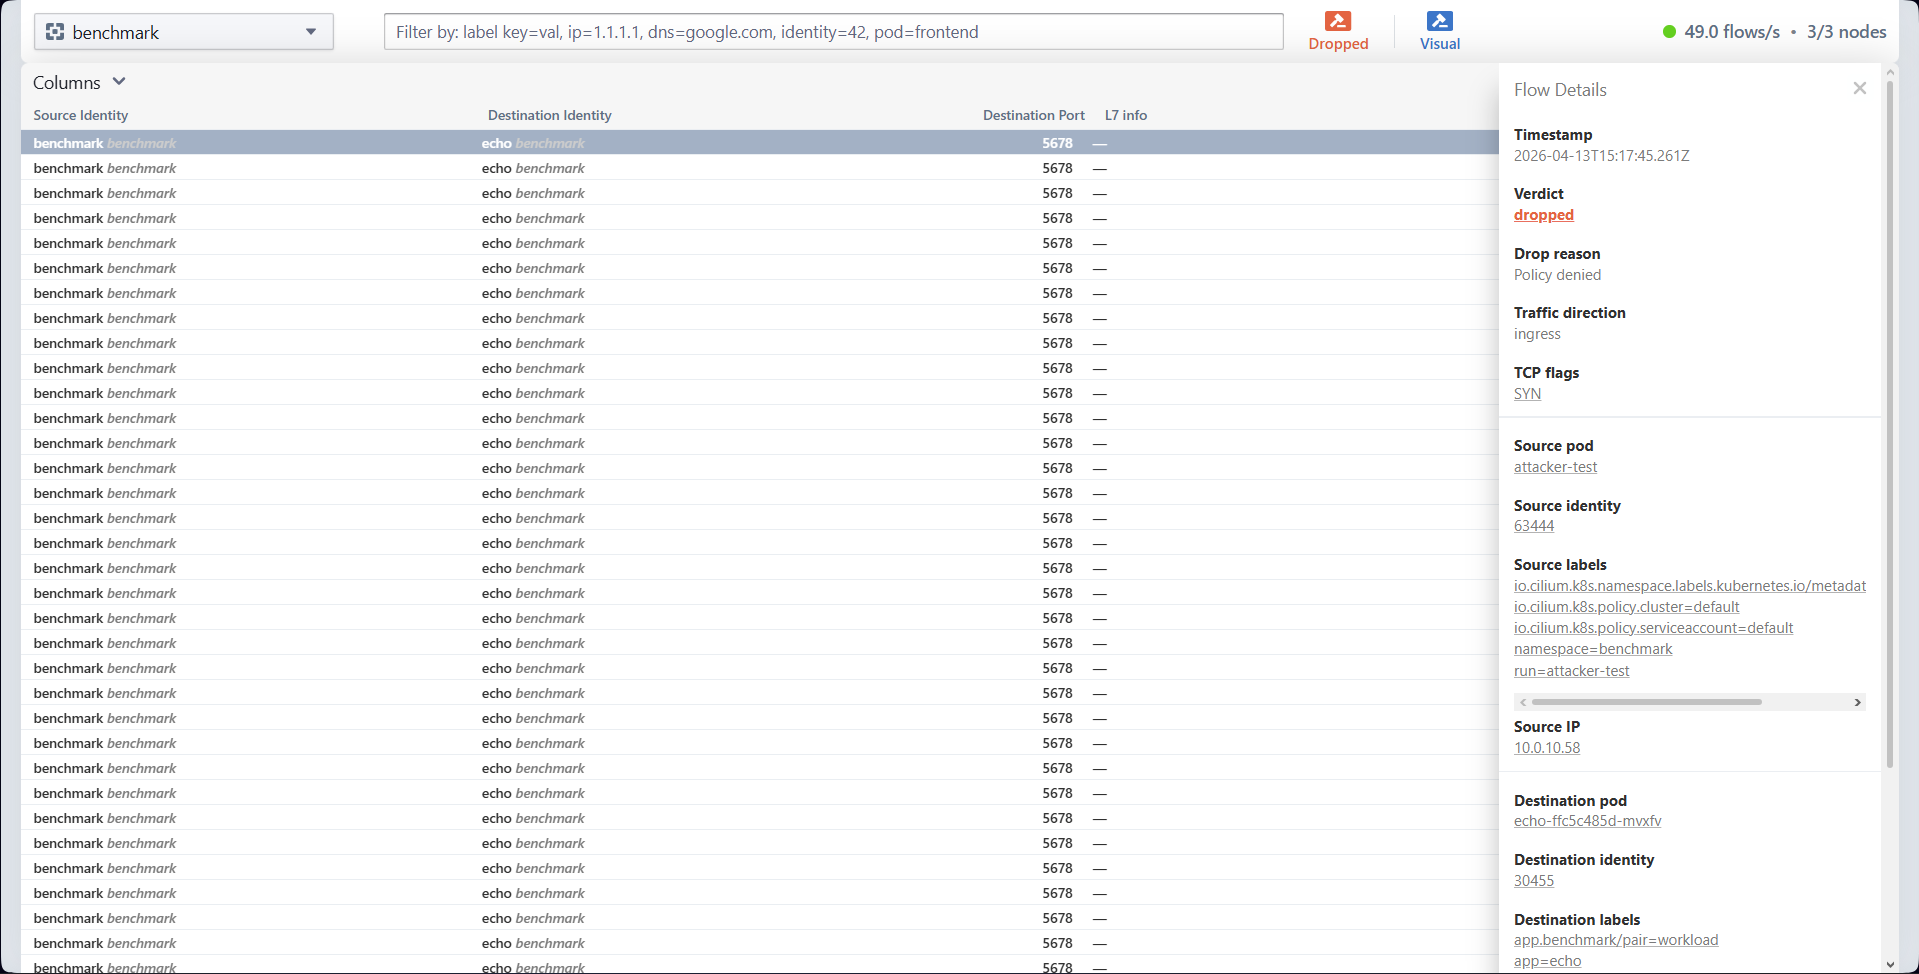
\includegraphics[width=0.86\textwidth]{../figures/hubble/fig13-hubble-deny-case-detail.png}
    \caption{Bằng chứng Hubble hỗ trợ cho S3 trong Mode B: forward-case với các flow được forwarded và manual deny-case với verdict policy denied; đây là evidence observability, không phải metric hiệu năng chính}
    \label{fig:s3-hubble-policy-evidence}
\end{figure}

\textbf{Kết luận.} Trong Mode B, với policy đơn giản và workload hiện tại, policy ON không tạo thay đổi p99 hoặc RPS đáng kể so với policy OFF. Kết luận này chỉ áp dụng cho setup đã đo và không nên khái quát cho policy phức tạp hơn.

\section{Độ lặp lại và tính ổn định}

Độ lặp lại giúp kiểm tra liệu kết luận có bị chi phối bởi một run cá biệt hay không. Hình~\ref{fig:repeatability-p99-dotplot} biểu diễn p99 của từng run cho các nhóm đại diện; mỗi điểm là một run thô, còn các vạch ngang ngắn là trung bình của nhóm, không phải khoảng tin cậy.

\begin{figure}[H]
    \centering
    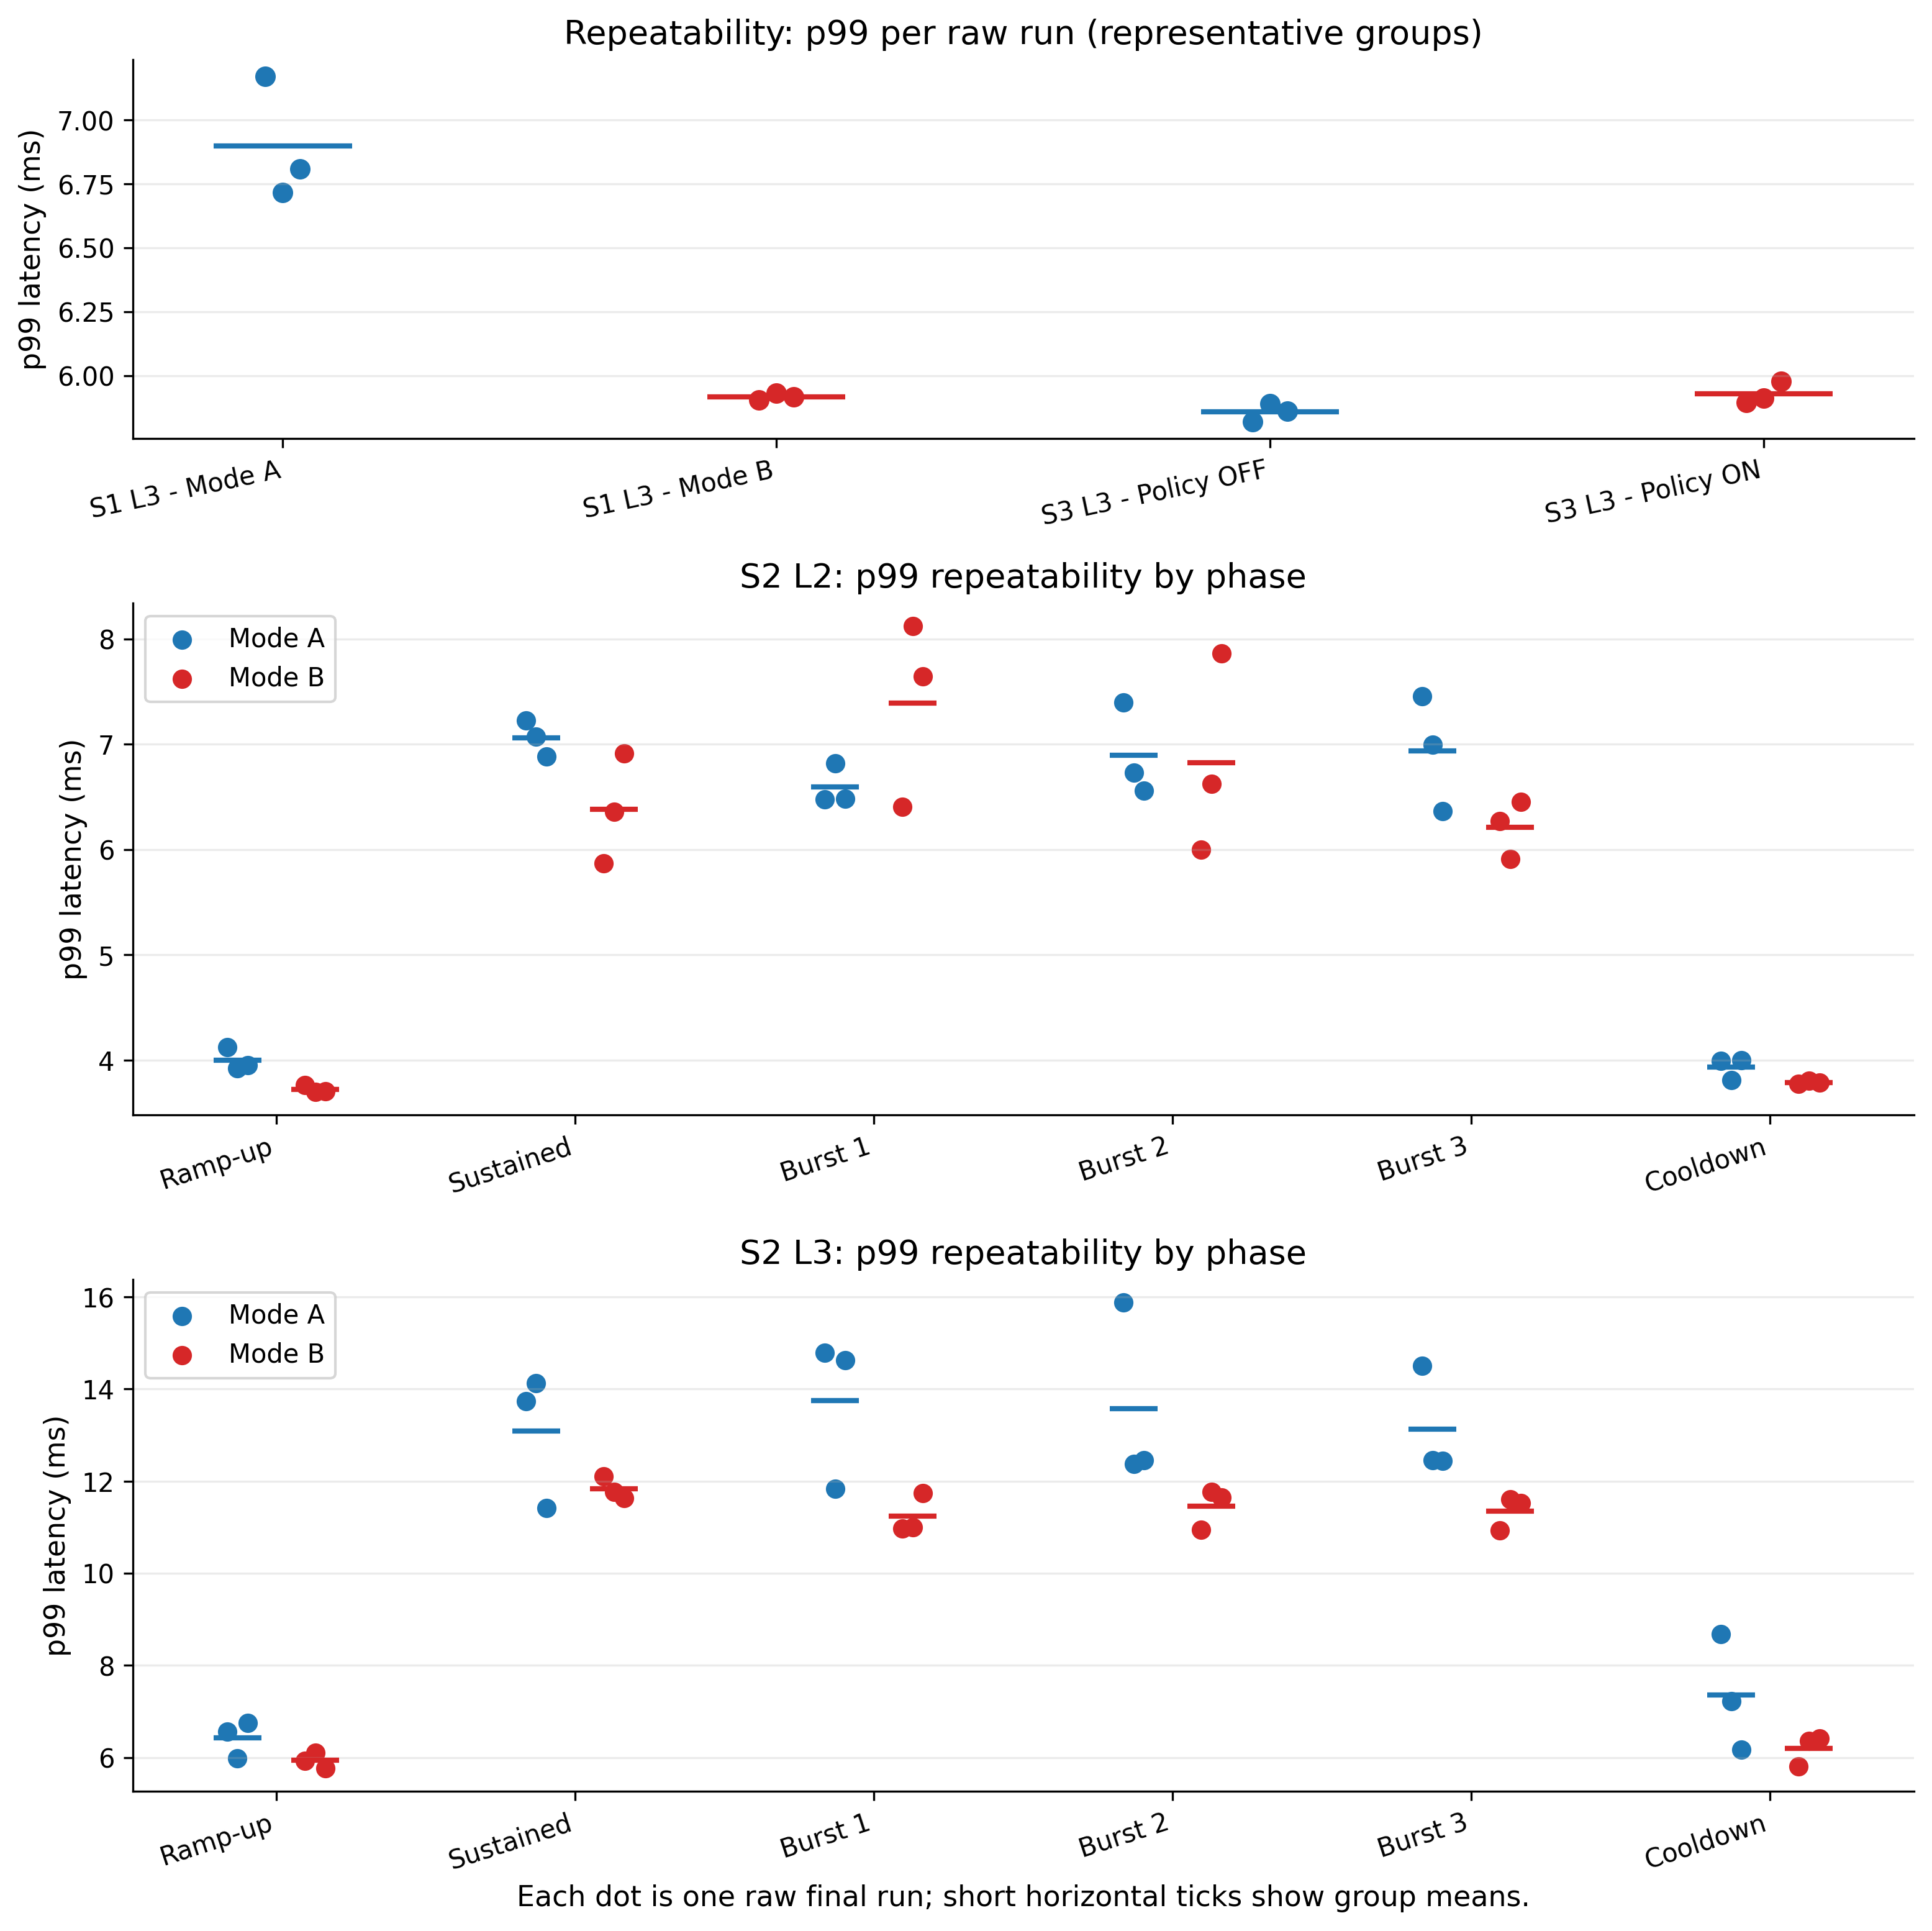
\includegraphics[width=0.90\textwidth]{../figures/thesis/fig-repeatability-p99-dotplot.png}
    \caption{Độ lặp lại p99 qua từng lần chạy; mỗi điểm là một run thô và vạch ngang ngắn là trung bình nhóm, không phải khoảng tin cậy}
    \label{fig:repeatability-p99-dotplot}
\end{figure}

\textbf{Phân tích.} CV\% mô tả dao động tương đối giữa các run. Ở S1 L3, Mode B vừa có p99 trung bình thấp hơn Mode A, vừa có CV thấp hơn; vì vậy, kết quả S1 có độ ổn định tốt hơn trong tập run hiện tại. Ở S3 L3, policy OFF và ON cũng có CV thấp, phù hợp với nhận định chênh lệch OFF/ON nhỏ.

Ngược lại, S2 biến động hơn do phase ngắn, burst và connection churn. Vì vậy, S1 và S3 có thể được diễn giải chắc hơn, còn S2 cần giữ ngôn ngữ thận trọng. Với \(n=3\), CV\% không làm tăng sức mạnh thống kê, nhưng giúp minh bạch chất lượng phép đo.

\textbf{Kết luận.} Độ lặp lại không thay thế kiểm định thống kê, nhưng giúp người đọc thấy nhóm nào ổn định hơn và nhóm nào cần diễn giải dè dặt. Đây là lý do mạch diễn giải của S1/S3 có thể chắc hơn, còn S2 nên được trình bày như xu hướng phụ thuộc pha.

\section{So sánh tổng hợp}

Bảng~\ref{tab:scenario-synthesis} tổng hợp vai trò của từng kịch bản, kết quả chính và caveat quan trọng nhất. Bảng này giúp liên kết các kịch bản thành một bức tranh chung, nhưng không thay thế phân tích chi tiết ở các mục trước.

\begin{table}[H]
\centering
\caption{Tổng hợp kết quả theo kịch bản}
\label{tab:scenario-synthesis}
\scriptsize
\setlength{\tabcolsep}{2.5pt}
\renewcommand{\arraystretch}{1.28}
\begin{tabularx}{\textwidth}{>{\raggedright\arraybackslash}p{2.0cm}>{\raggedright\arraybackslash}p{3.0cm}>{\raggedright\arraybackslash}X>{\raggedright\arraybackslash}p{3.0cm}}
\toprule
\textbf{Kịch bản} & \textbf{Mục tiêu} & \textbf{Kết quả chính} & \textbf{Caveat chính} \\
\midrule
Hiệu chuẩn & Chọn mức tải cuối & L1=100, L2=400, L3=800 QPS; L3 là tail-spike load, chưa phải saturation tuyệt đối & Error rate 0\% không có nghĩa là không có stress \\
S1 & So sánh Mode A và Mode B dưới tải ổn định & Mode B có p99 thấp hơn, rõ nhất ở L2 và L3 & L1 không significant; không khái quát ngoài môi trường đo \\
S2 & Kiểm tra burst, churn và hành vi theo pha & L3 cho xu hướng Mode B thấp hơn ở toàn bộ pha; L2 có kết quả pha trộn & Variance cao; Burst 1 L2 là ngoại lệ \\
S3 & Đo policy OFF/ON trong Mode B & Policy ON không làm p99 hoặc RPS thay đổi đáng kể trong dataset hiện tại & Chỉ áp dụng cho policy đơn giản và traffic hiện tại \\
Độ lặp lại & Kiểm tra độ ổn định giữa các run & S1/S3 ổn định hơn; S2 biến động hơn & \(n=3\) vẫn là giới hạn quan trọng \\
\bottomrule
\end{tabularx}
\end{table}

Nhìn tổng thể, S1 cung cấp bằng chứng sạch nhất về khác biệt datapath trong điều kiện ổn định. S2 cho thấy khác biệt phụ thuộc vào pha và mức tải. S3 tách riêng câu hỏi chi phí policy trong Mode B và cho thấy overhead quan sát được nhỏ với policy đơn giản. Độ lặp lại giúp xác định nhóm kết quả nào có thể viết chắc hơn và nhóm nào chỉ nên xem là xu hướng.

\section{Phân tích theo RQ1, RQ2 và RQ3}

\subsection{RQ1: Mode B có cải thiện latency trong tải ổn định so với Mode A không?}

Câu trả lời ngắn gọn là có bằng chứng ủng hộ, đặc biệt tại L2 và L3. Trong S1, Mode B có p99 trung bình thấp hơn Mode A ở cả ba mức tải; L2 và L3 được đánh dấu significant, còn L1 chỉ nên xem là xu hướng. Vì vậy, trong điều kiện steady-state của benchmark hiện tại, Mode B cho thấy lợi thế tail latency rõ hơn ở tải trung bình và tải cao.

\subsection{RQ2: Khác biệt giữa hai mode thay đổi thế nào dưới burst và connection churn?}

Câu trả lời là khác biệt phụ thuộc vào pha và mức tải. Tại L2, Mode B có xu hướng tốt hơn ở nhiều pha nhưng Burst 1 là ngoại lệ. Tại L3, Mode B có p99 trung bình thấp hơn ở toàn bộ pha, đặc biệt trong các pha burst, nhưng chưa significant. Vì vậy, S2 ủng hộ nhận định Mode B có thể có lợi thế tail latency dưới tải cao và workload động, nhưng chưa đủ để khẳng định tốt hơn ở mọi pha.

\subsection{RQ3: Bật NetworkPolicy trong Mode B có tạo chi phí đáng kể không?}

Câu trả lời là trong tập dữ liệu hiện tại, chi phí quan sát được là nhỏ. Trong S3, policy ON không làm RPS giảm đáng kể và p99 chỉ thay đổi rất nhỏ so với OFF. Error rate bằng 0\% cho thấy workload hoàn tất thành công, nhưng không chứng minh overhead bằng không. Kết luận này chỉ áp dụng cho policy đơn giản và allowed traffic trong benchmark hiện tại.

\section{Tổng kết chương}

Chương này đã trình bày kết quả benchmark theo logic kịch bản: hiệu chuẩn tải, S1, S2, S3 và độ lặp lại. Mode B có lợi thế p99 rõ nhất trong S1 ở L2/L3; trong S2, xu hướng có lợi cho Mode B rõ hơn ở L3 nhưng phụ thuộc pha; trong S3, NetworkPolicy đơn giản trong Mode B không tạo overhead p99/RPS đáng kể trong dataset hiện tại.

Các kết luận trên cần được đọc trong phạm vi thực nghiệm của đề tài: EKS, 3 worker nodes \texttt{m5.large}, workload Fortio/HTTP echo, các mức tải L1/L2/L3, số lần lặp nhỏ và policy đơn giản. Chương 5 sẽ dùng các kết quả này để tổng hợp đóng góp, nêu giới hạn nghiên cứu và đề xuất hướng mở rộng.
